%%____________________________________________________________________________||
\section{Systematic uncertainties in the \mht dimension}
\label{sec:mhtTemplate}

The estimate of the number of events per (\njet,\nb,\scalht) bin,
integrated over \mht, is determined from data control samples, with
the associated systematic error determined from closure tests
described in Section \ref{sec:syst-from-closure}. This section
describes the method used to determine the systematic uncertainties in
the distribution of events according to \mht. A data driven approach is
utilised where the level of closure in the control regions is used
to determine the maximum deviation expected in the signal region.

When looking at the \mht dimension inclusively there are
large theoretical uncertainties that originate from mixing events
at different scales. However, if a a variable, such as \ht, 
that is strongly correlated with the scale of the event 
is used to 'set the scale' these uncertainties can be mitigated.
In \ref{valid8} the 8 TeV data will be used to show that binning in
\ht elminates bias in the data and MC agreement in the control regions. 
In \ref{sadf} this will then be used to extract systematic template 
variations in the signal region. Finally, in \ref{asdf} results for the
expected systematic for Run 2 will be shown.


% extent to which the control regions can constrain this bias 
% to the flat hypothesis
%Motivated by the inclusive distribution, a linear bias is assumed.

\section{Validation with 8 \TeV Data}
\label{valid8}
In previous versions of this analysis three control regions
were used: \mj, \mmj and \gj. In Figure~\ref{fig:linearMotiv} the data/MC 
distribution against \mht for the control region selection 
(detailed in \cite{CMS_AN_2013-366}) is shown inclusive 
in \ht and categories. By fitting a second order orthogonal polynomial
it can be seen that in each case the quadratic term is small and consistent
with zero. Motivated by this a linear function will be used to measure
the level of bias remaining when the \mht dimension is binned in \mht. 
As the normalisation systematic is dealt with seperately the normalisation
of the MC is set to that of the data when fitting alternative templates.

\begin{figure}[h!]
  \centering
  \subfigure[\gj]{
    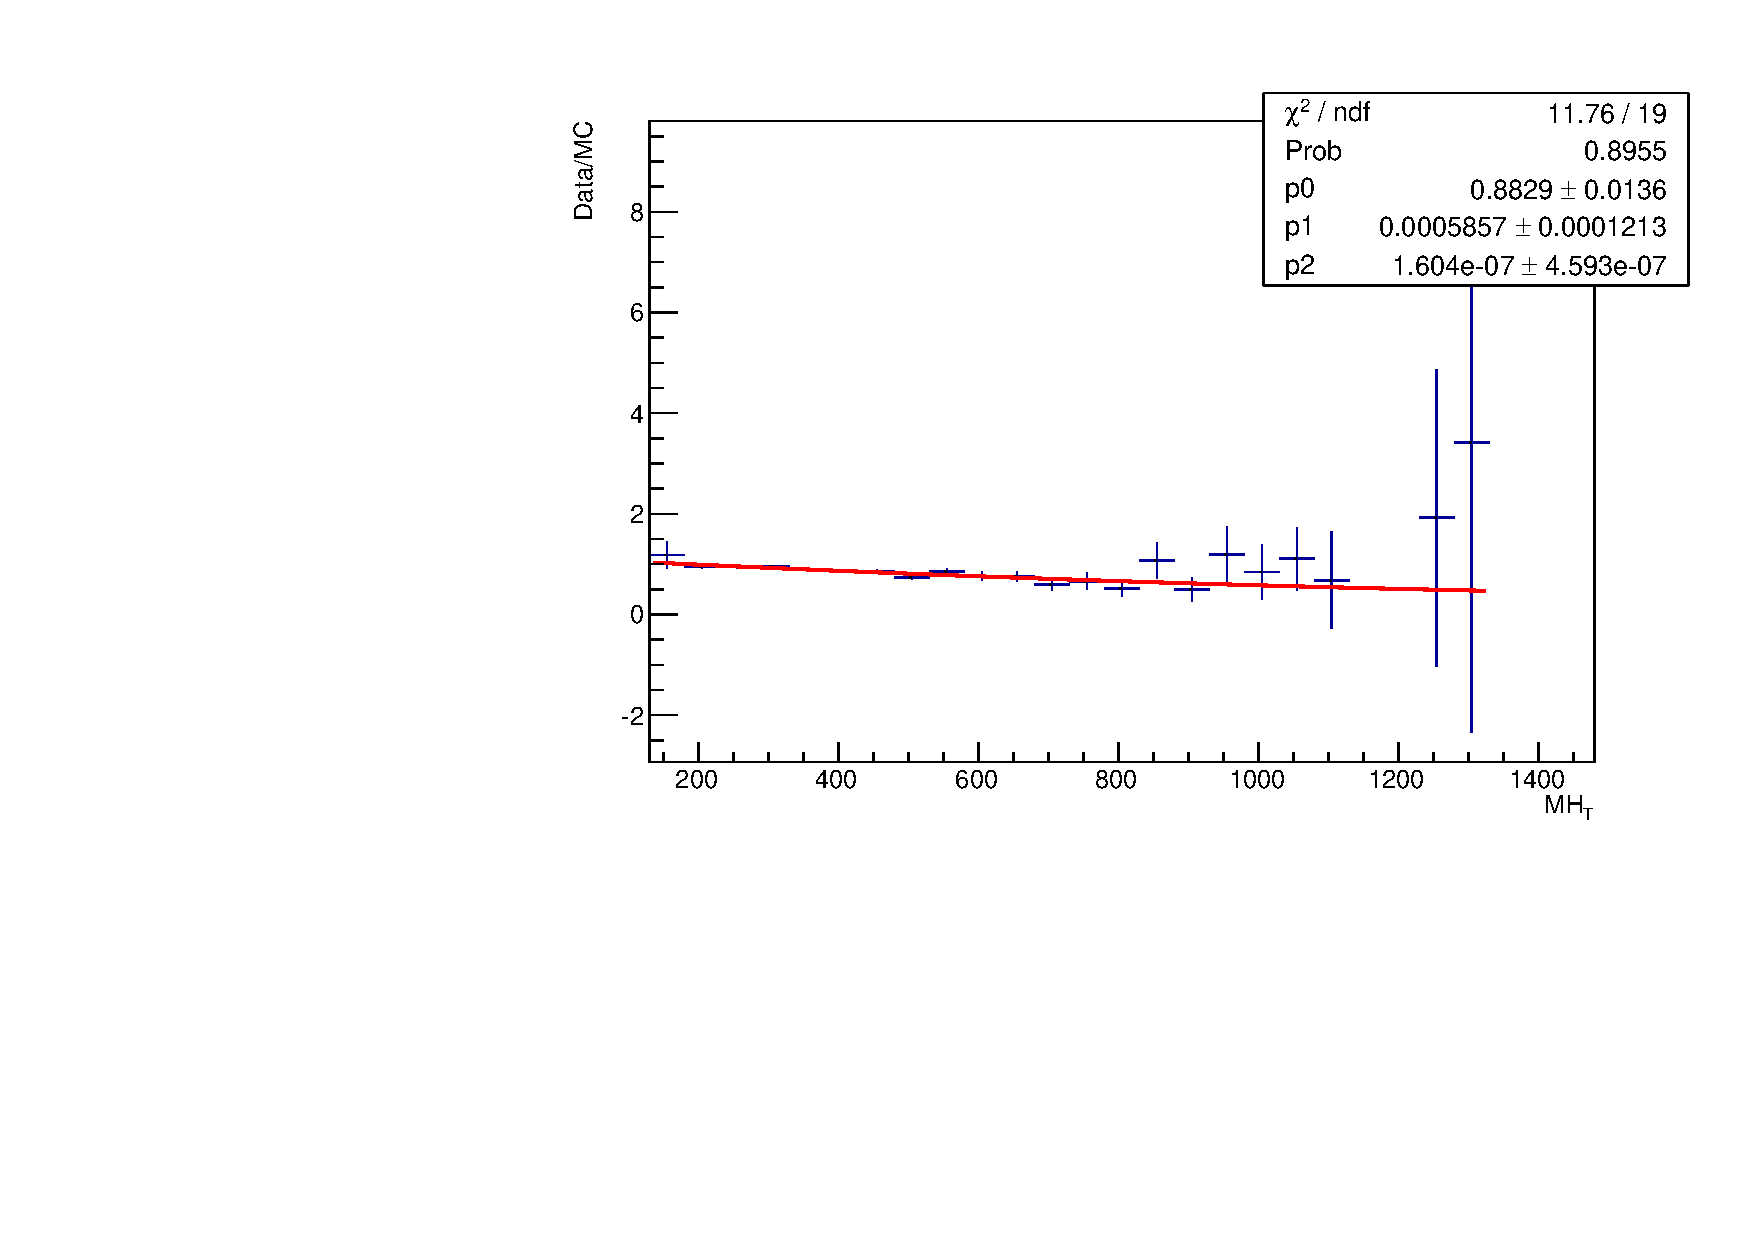
\includegraphics[width=0.5\textwidth]{figures/template/quadratic/mht_Inc_Inc_ht_Inc_SinglePhoton_Quadratic.pdf}
  }~~
  \subfigure[\mmj]{
    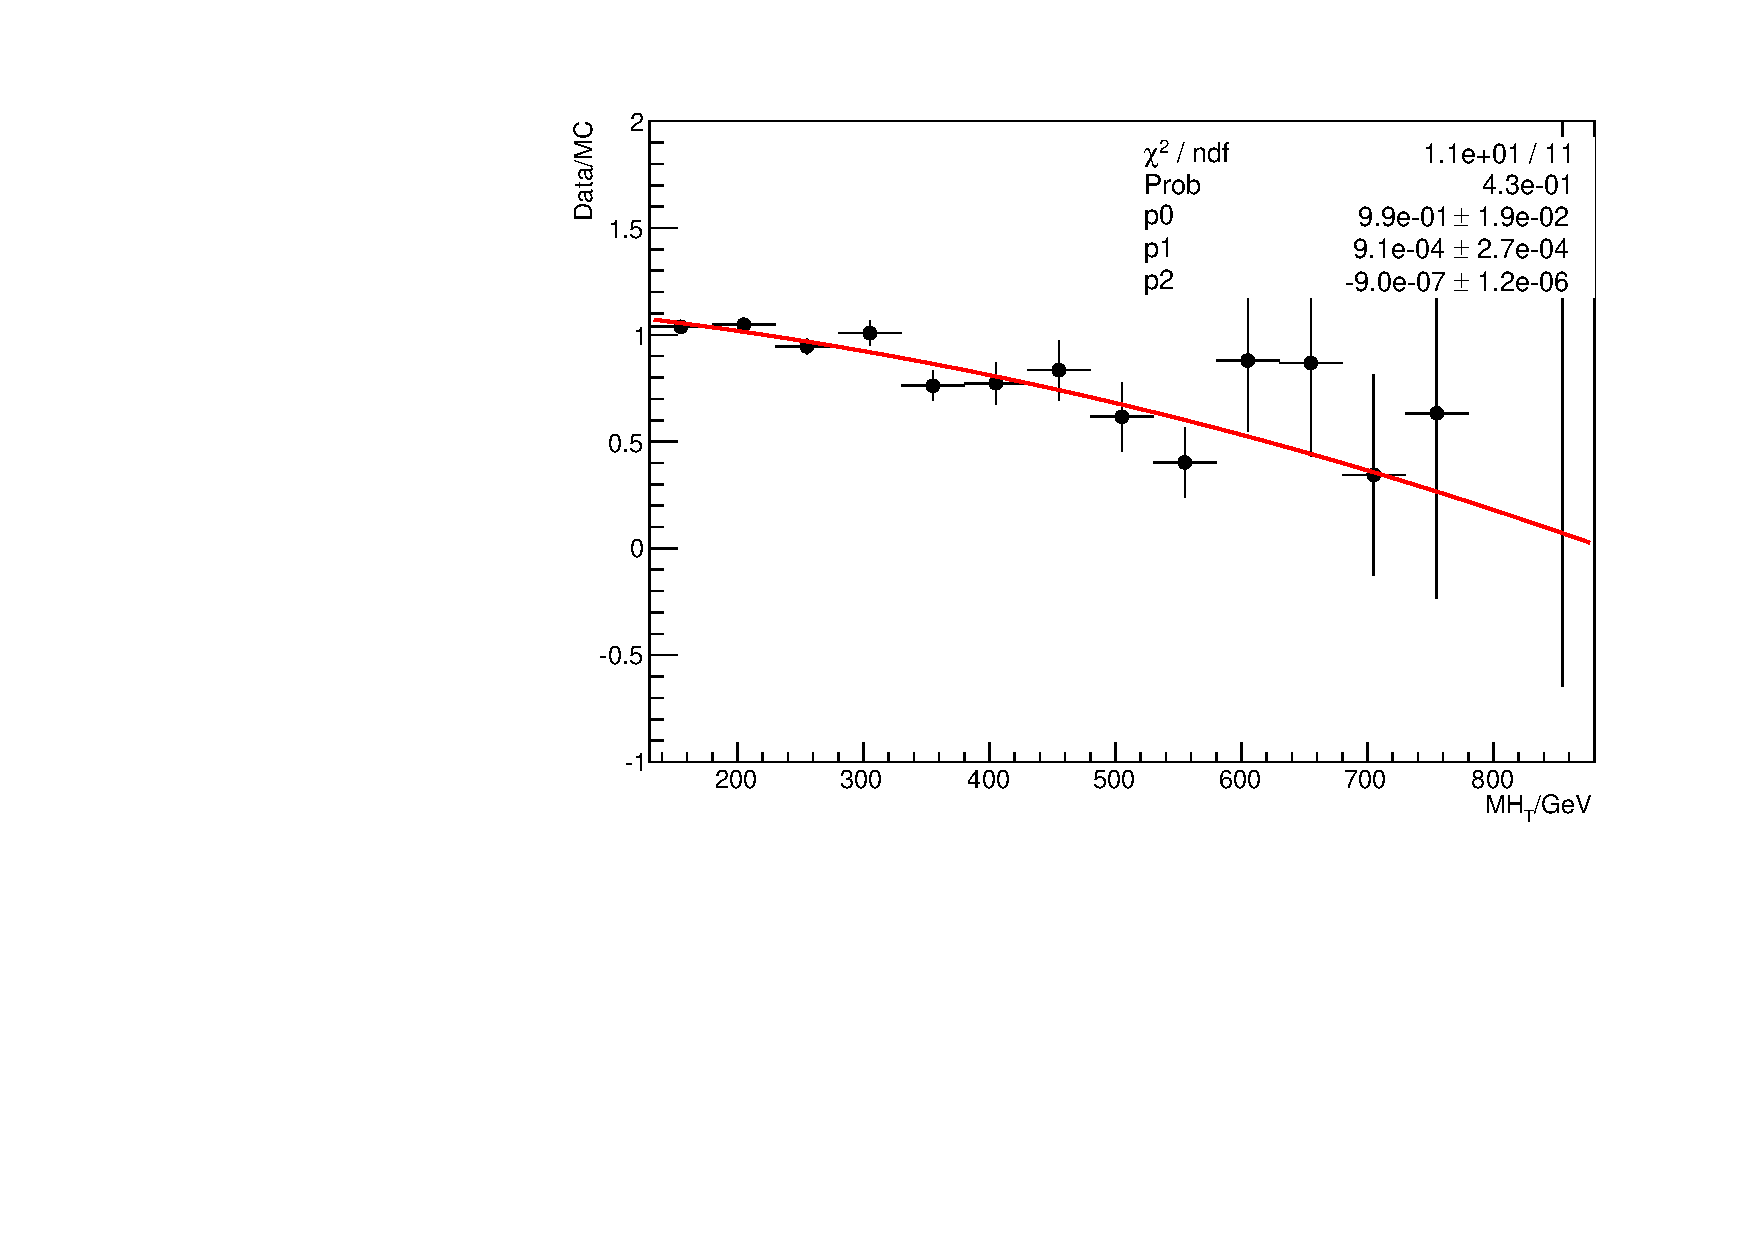
\includegraphics[width=0.5\textwidth]{figures/template/quadratic/mht_Inc_Inc_ht_Inc_DoubleMu_Quadratic.pdf}
  }\\
  \subfigure[\mj]{
    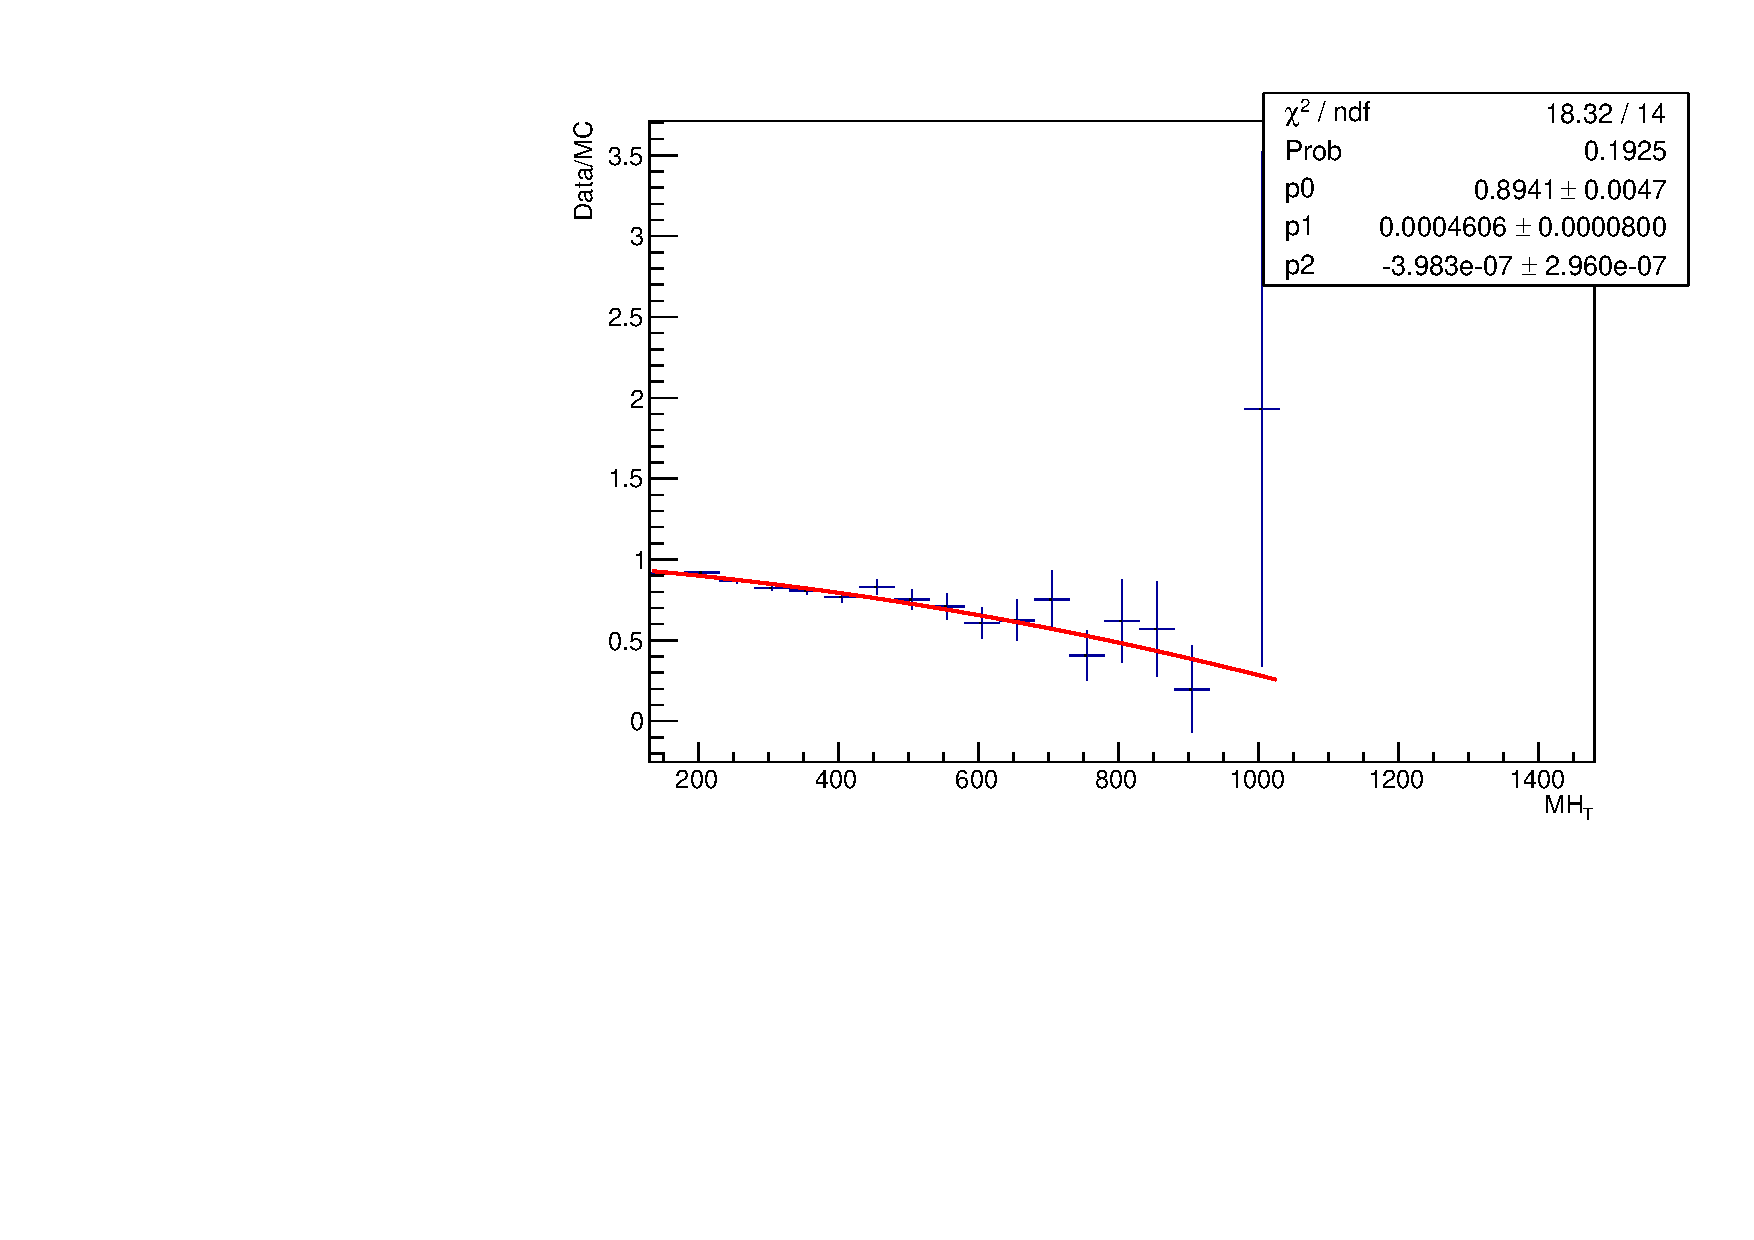
\includegraphics[width=0.5\textwidth]{figures/template/quadratic/mht_Inc_Inc_ht_Inc_SingleMu_Quadratic.pdf}
  }~~
  \\
  \caption{\label{fig:linearMotiv} 
  The data/MC distribution against \mht for an inclusive selection on category and \ht
  showing the results of a quadratic fit. There is a clear bias
  in the linear component while the quadratic component is consistent with zero.
}
\end{figure}

By anchoring the scale using binning in the \ht dimension the remaining
bias should be negligible. In Figures~\ref{fig:linearFits0bLe3} and \ref{fig:linearFits0bGe4} 
example fits of an orthogonal linear function to the data/MC ratio 
are shown for the three control regions. Comparing to the inclusive distribution 
the linear component can be seen to be much more compatible with the null, 
zero bias hypothesis. In order to formalise this assertion 
the pull of the linear component from zero is calculated.
This pull distribtuion is shown for each of the three control regions in
in Figure~\ref{fig:pulls} and can be see in each case to have mean and sigma
consistent with zero and one respectively. This supports the zero
bias hypothesis. Figure~\ref{fig:frenchFlagPull} shows the distribution of the pulls 
in category and \ht bins. Those anchored by \ht are consistent
with zero (including inclusive categories) while fits inclusive in \ht
show very large pulls. This shows as expected the \ht anchoring
is critical for removing bias in the \mht dimension.  

\begin{figure}[h!]
  \centering
  \subfigure[\gj]{
    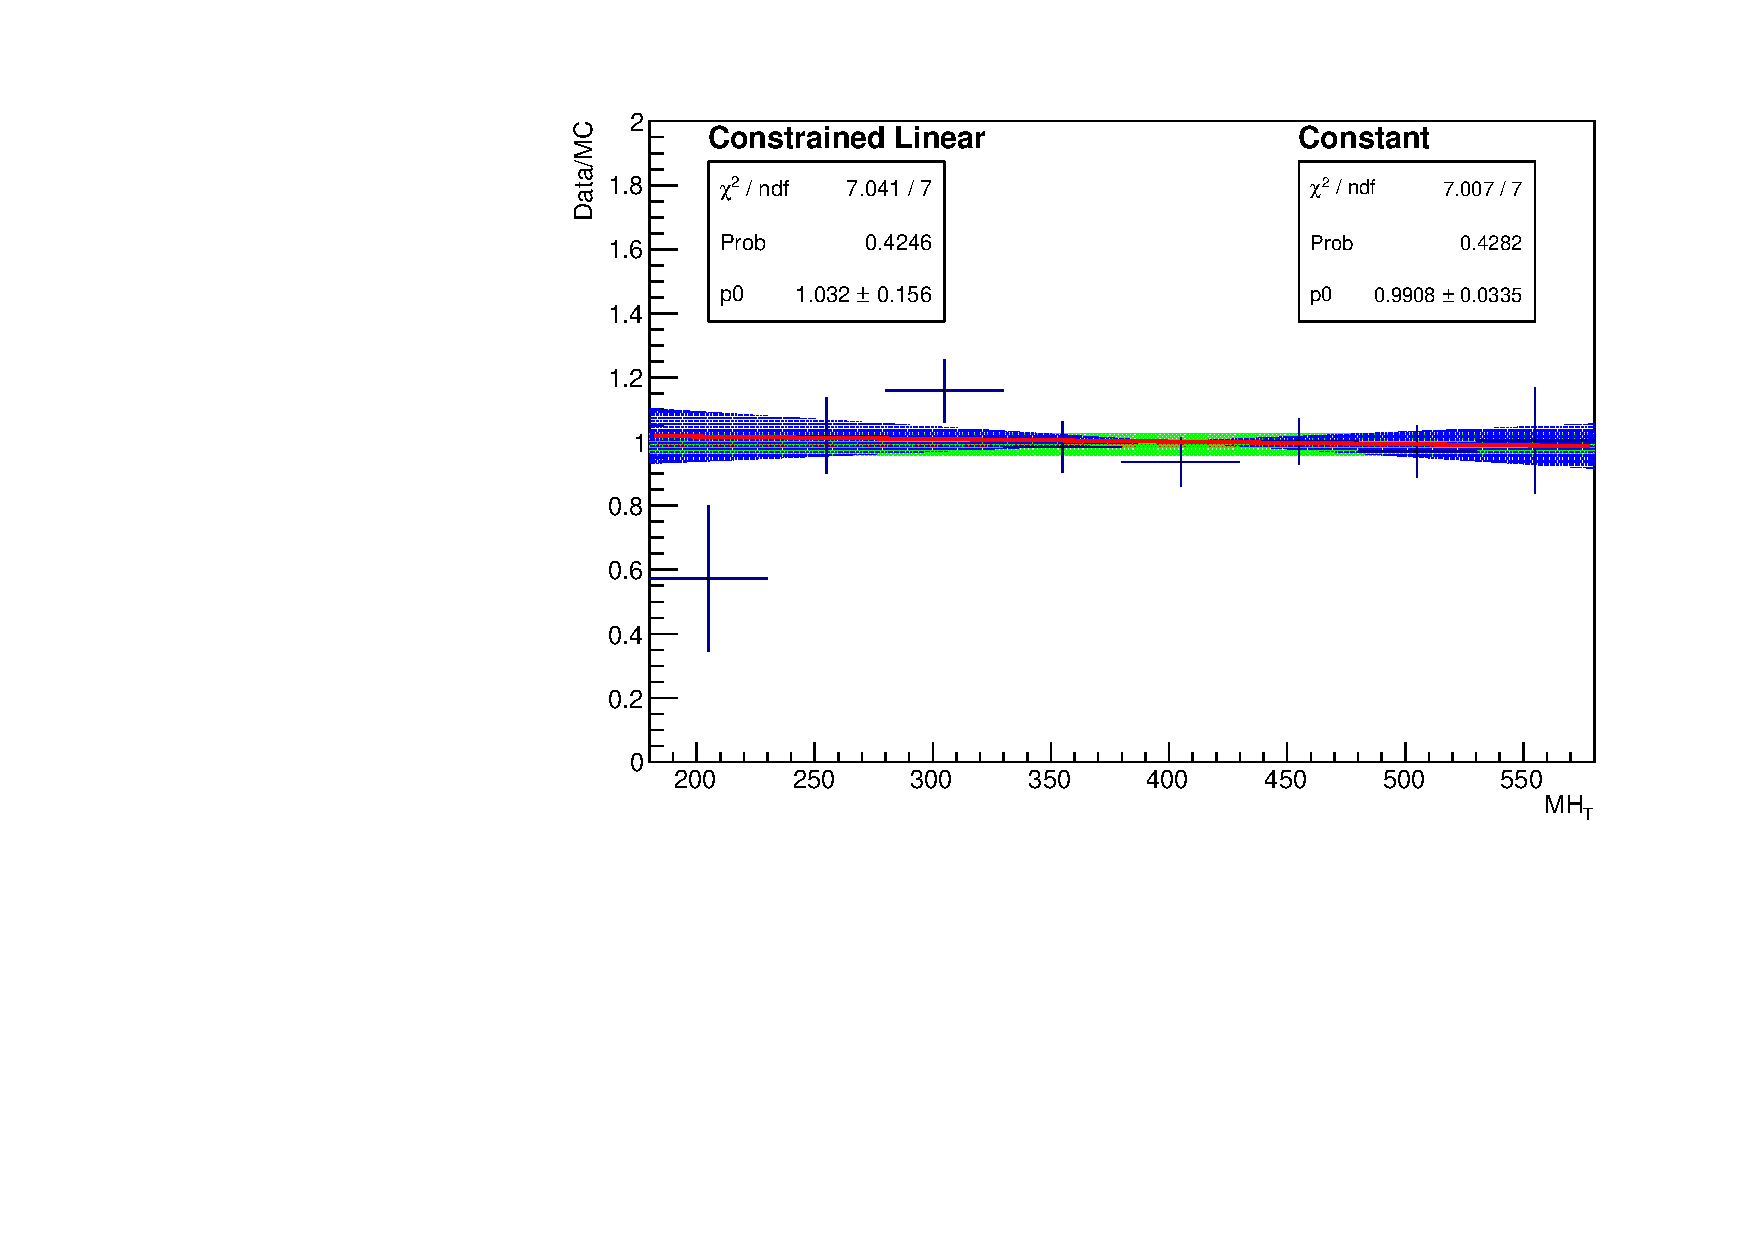
\includegraphics[width=0.5\textwidth]{figures/template/linear/mht_eq0b_le3j_ht_475_575_SinglePhoton.pdf}
  }~~
  \subfigure[\mmj]{
    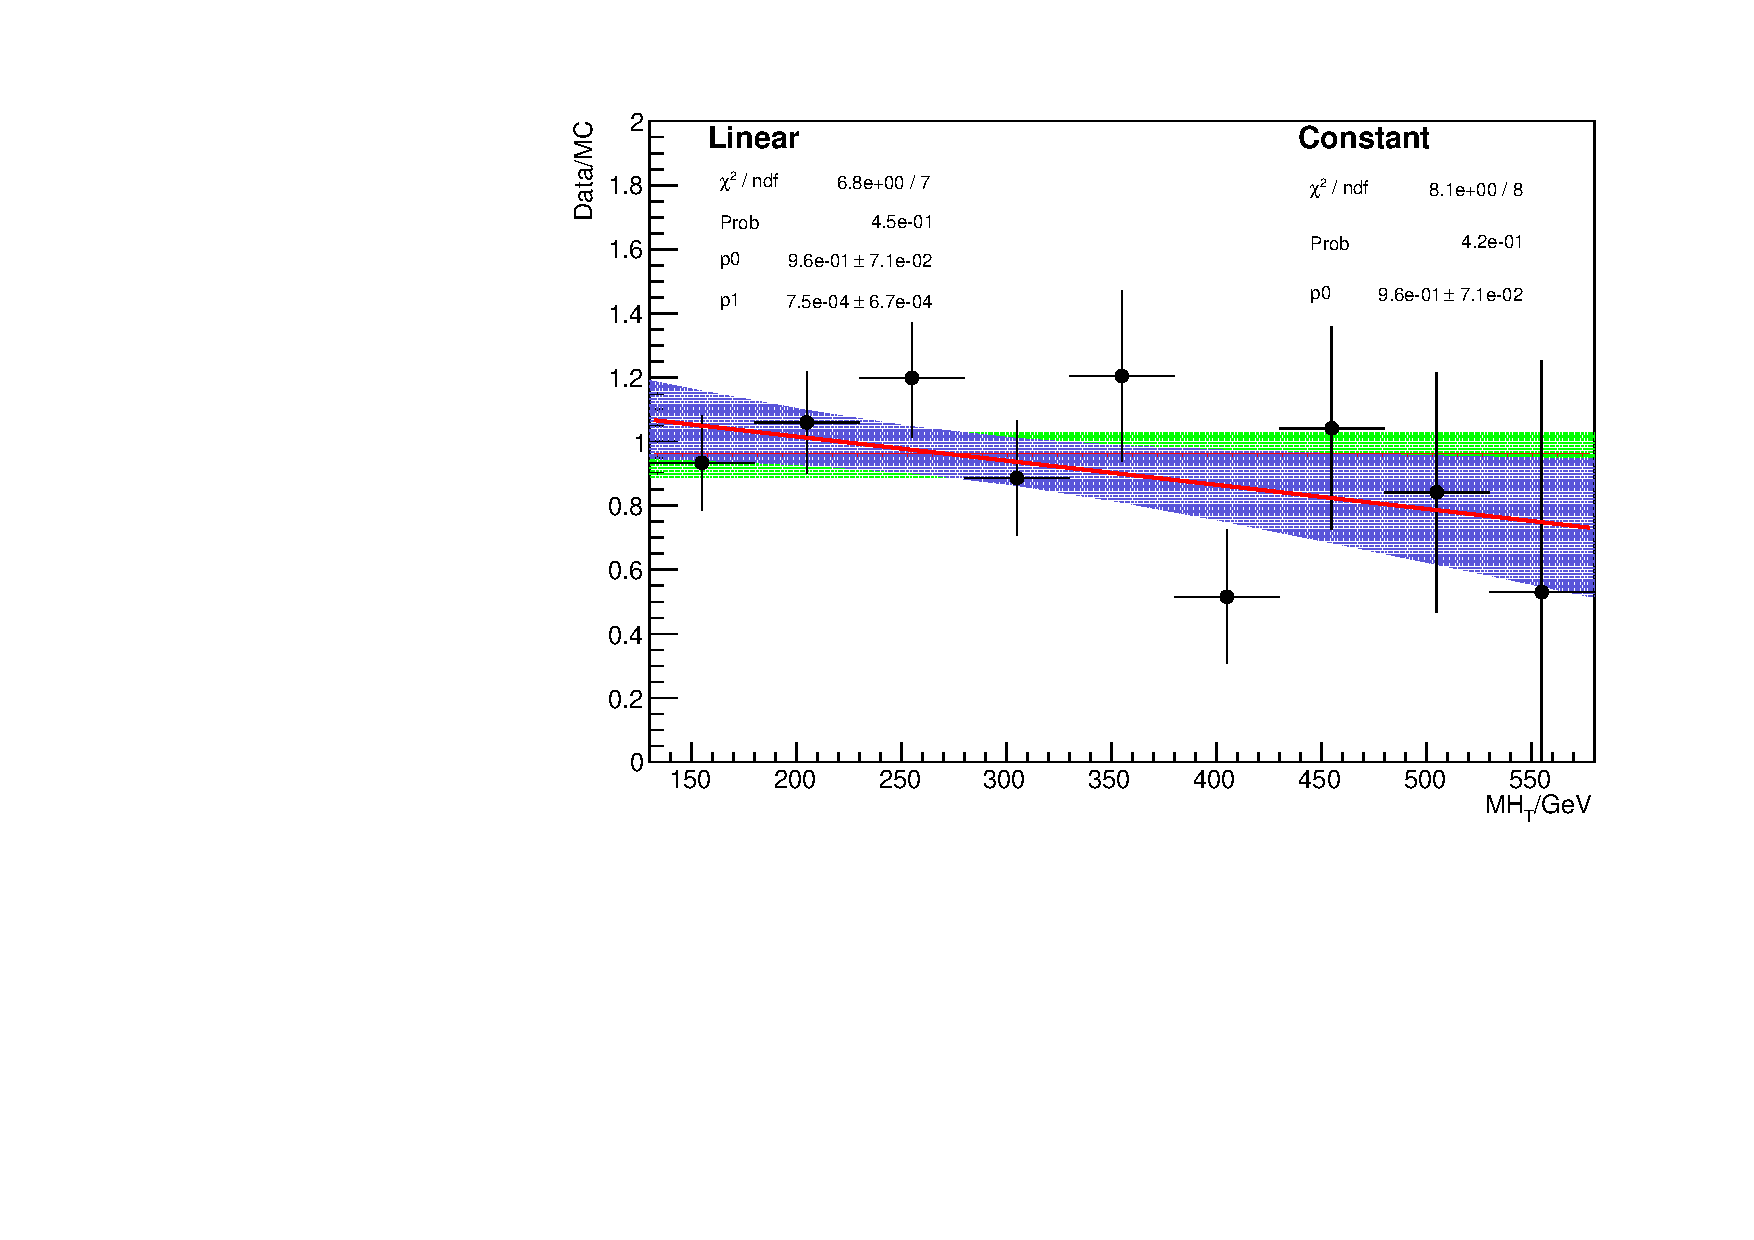
\includegraphics[width=0.5\textwidth]{figures/template/linear/mht_eq0b_le3j_ht_475_575_DoubleMu.pdf}
  }\\
  \subfigure[\mj]{
    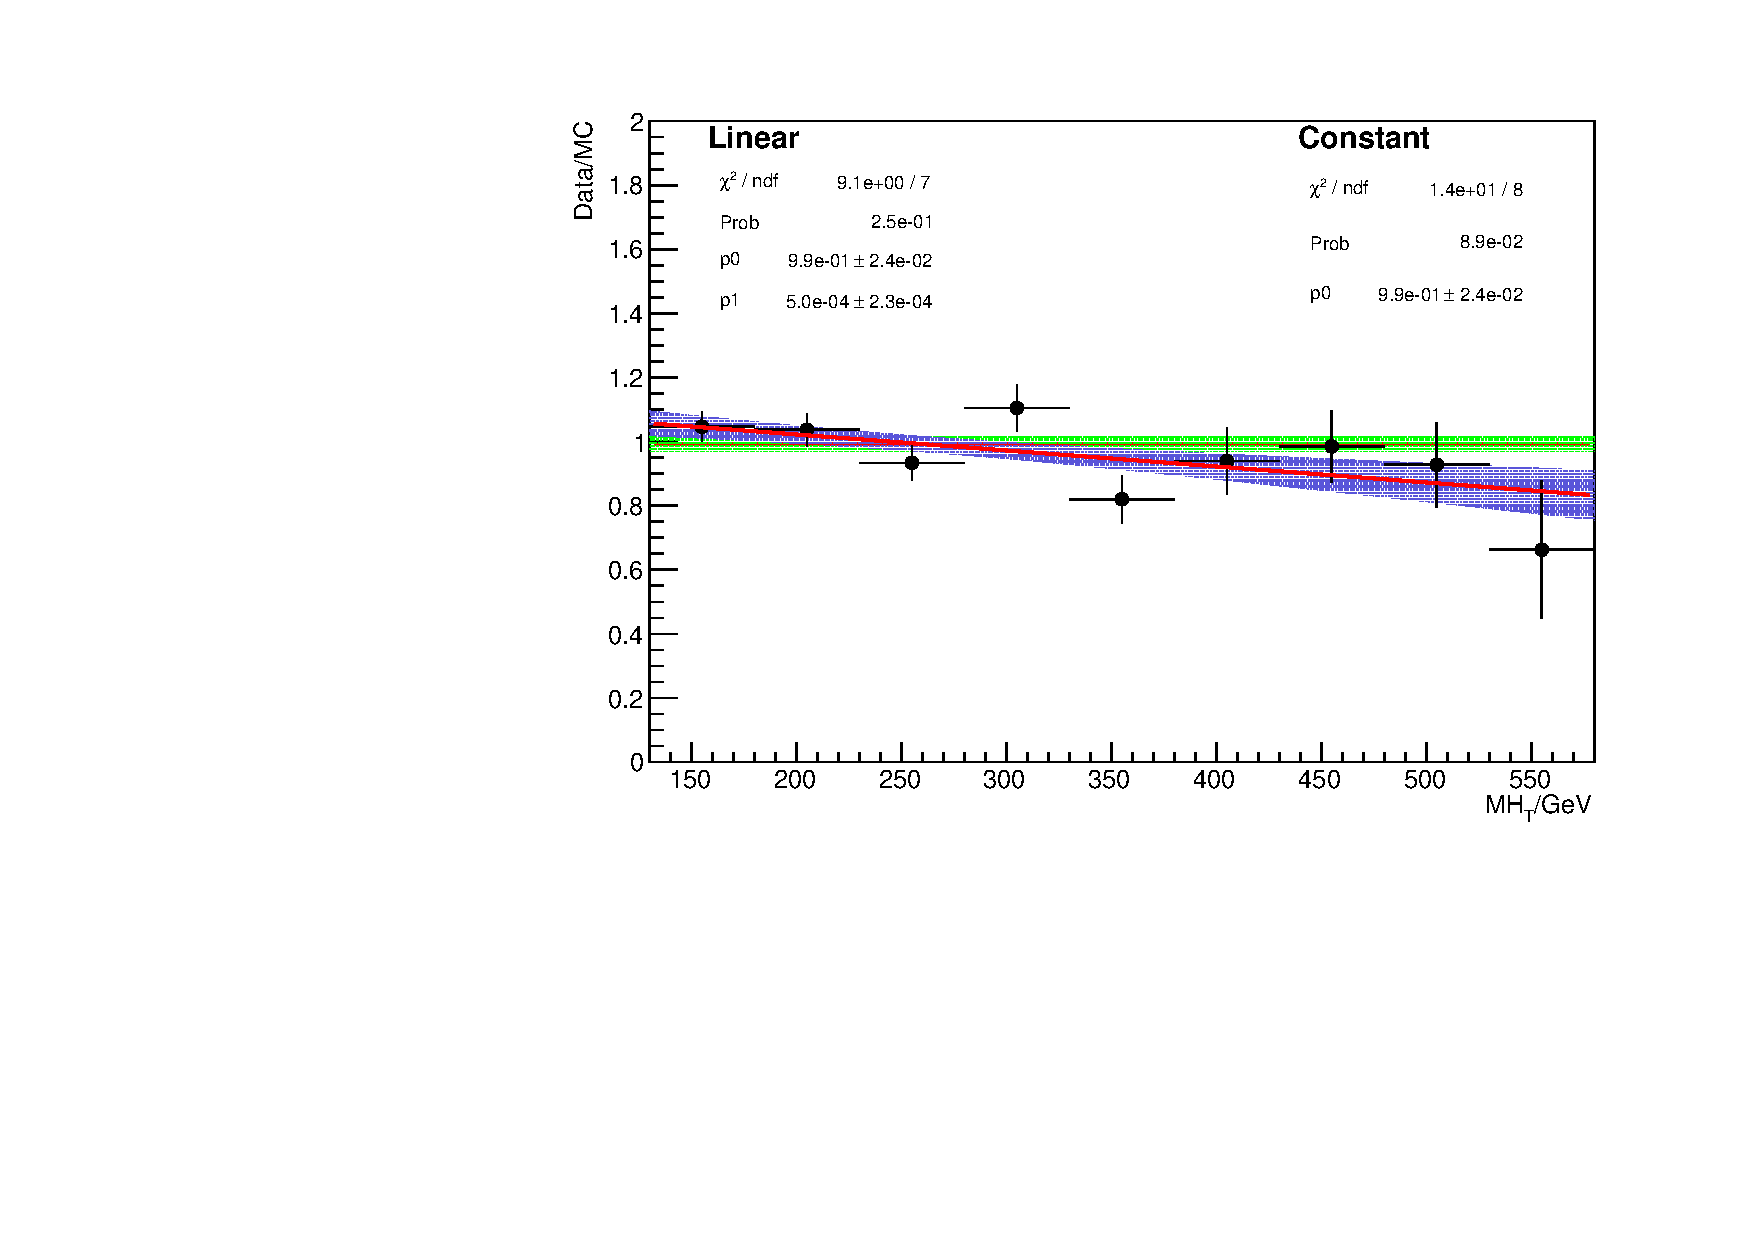
\includegraphics[width=0.5\textwidth]{figures/template/linear/mht_eq0b_le3j_ht_475_575_SingleMu.pdf}
  }~~
  \\
  \caption{\label{fig:linearFits0bLe3} 
  The data/MC distribution against \mht for the 0b, $\le3$j category and \ht 475-575\GeV bin.
  The large linear bias in the linear component seen in \ref{fig:linearMotiv} is
  largely mitigated.
}
\end{figure}

\begin{figure}[h!]
  \centering
  \subfigure[\gj]{
    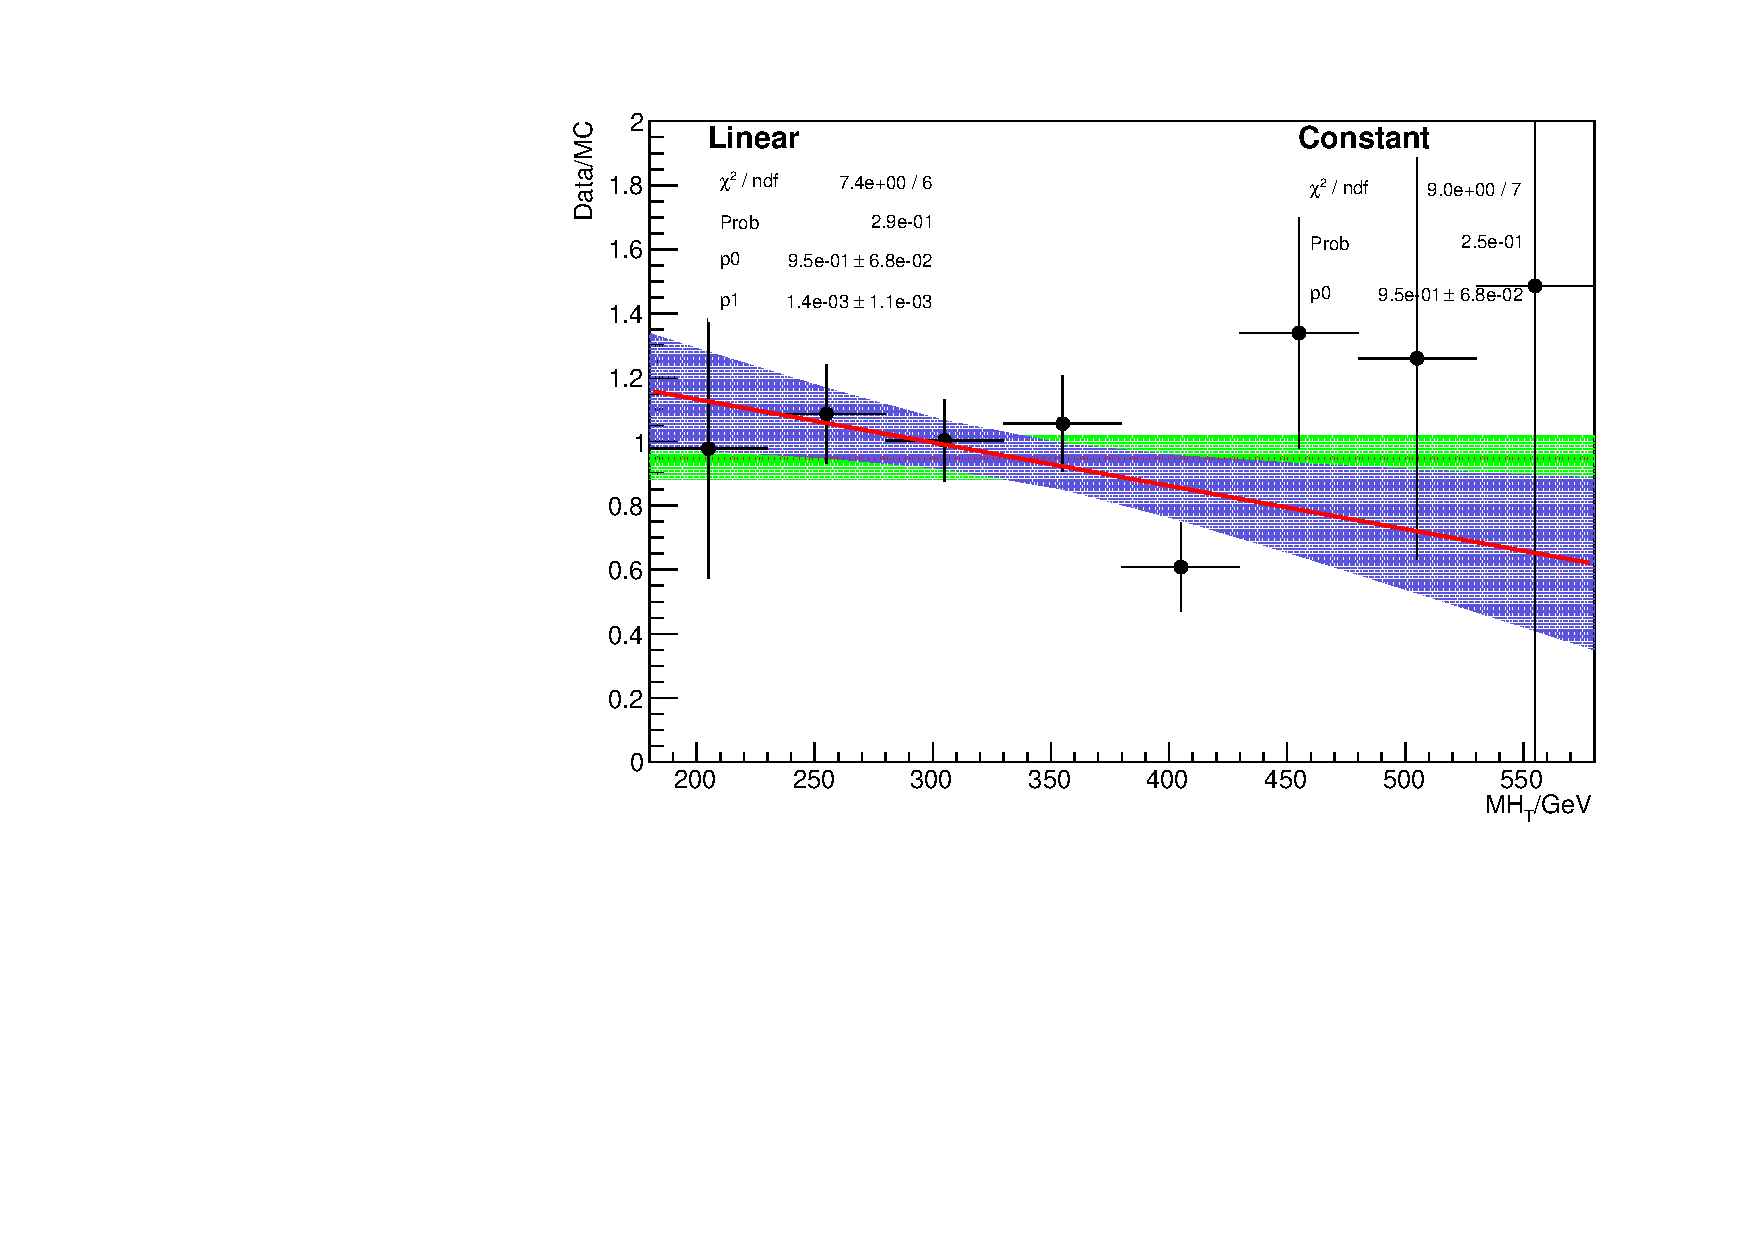
\includegraphics[width=0.5\textwidth]{figures/template/linear/mht_eq0b_ge4j_ht_475_575_SinglePhoton.pdf}
  }~~
  \subfigure[\mmj]{
    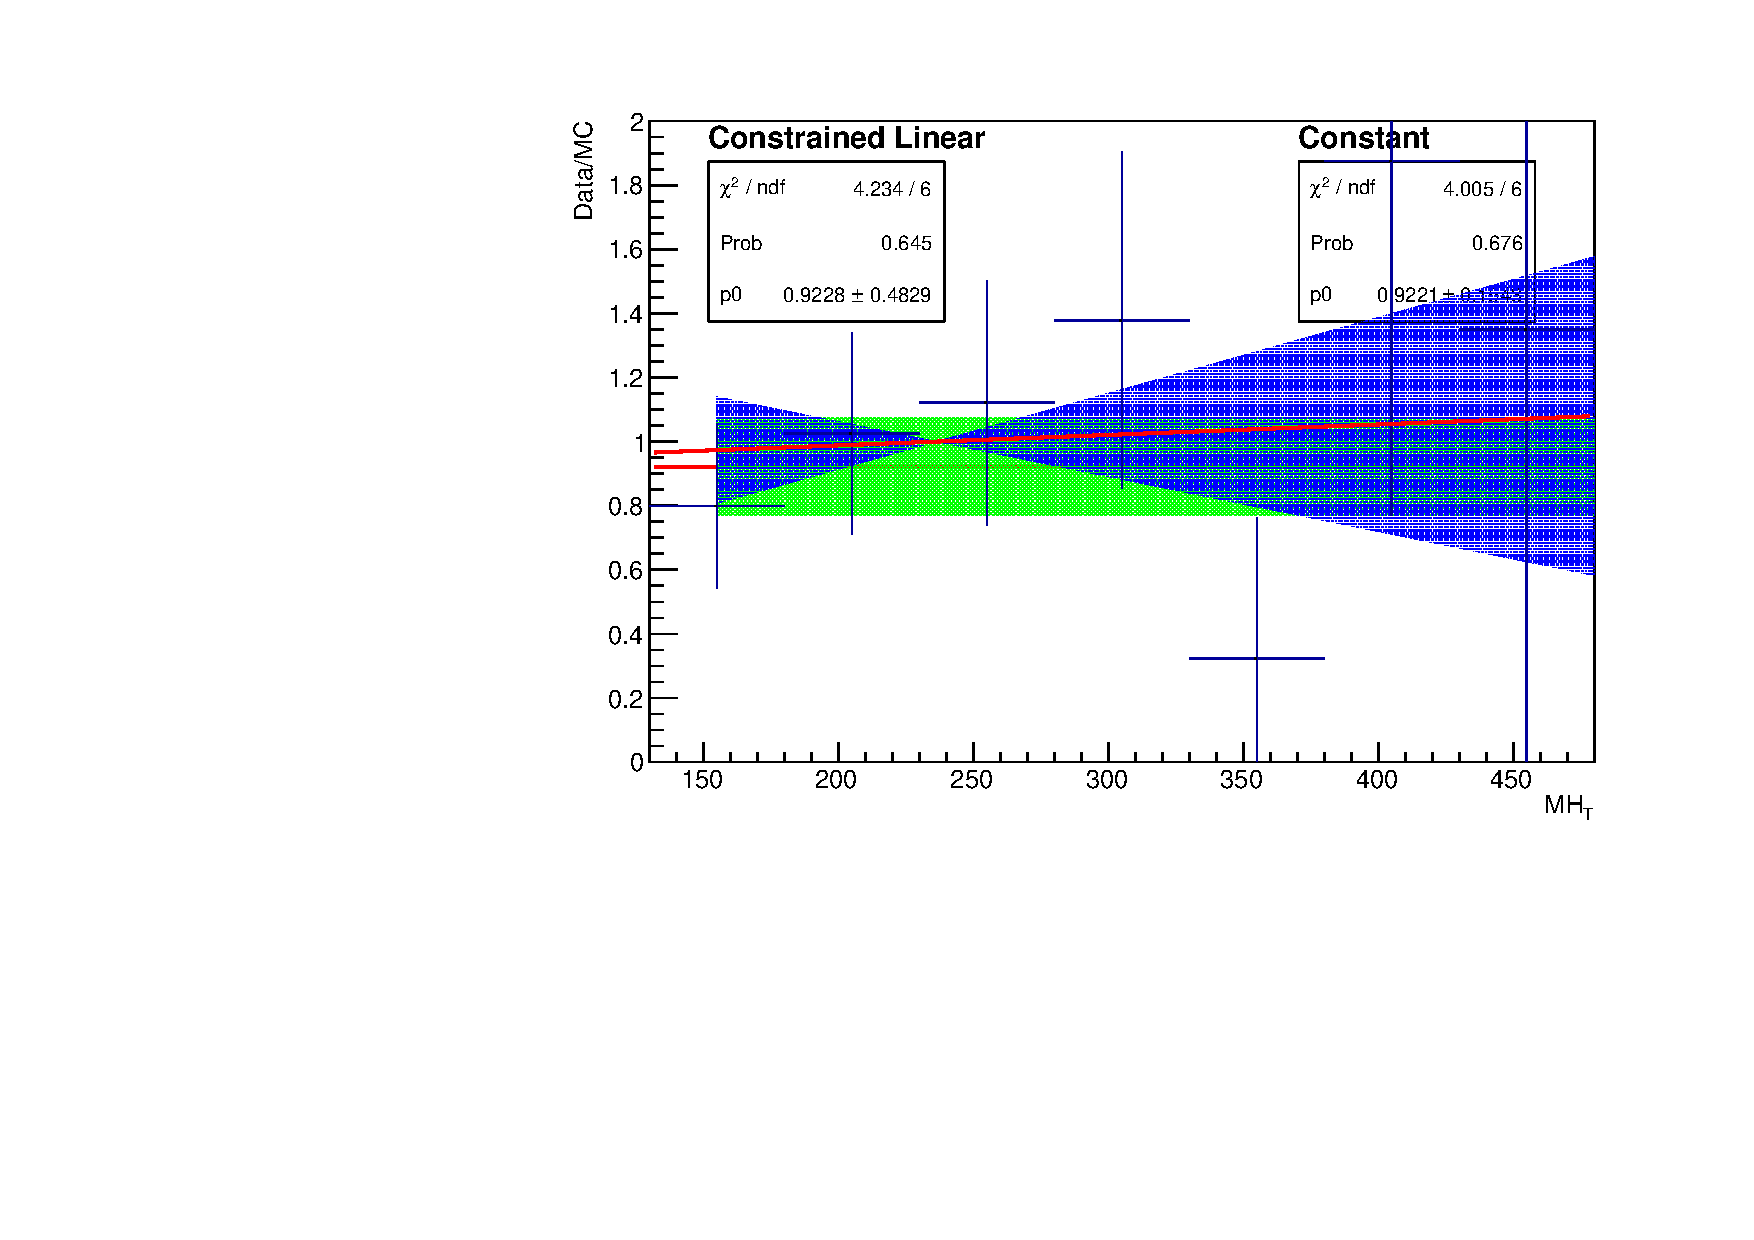
\includegraphics[width=0.5\textwidth]{figures/template/linear/mht_eq0b_ge4j_ht_475_575_DoubleMu.pdf}
  }\\
  \subfigure[\mj]{
    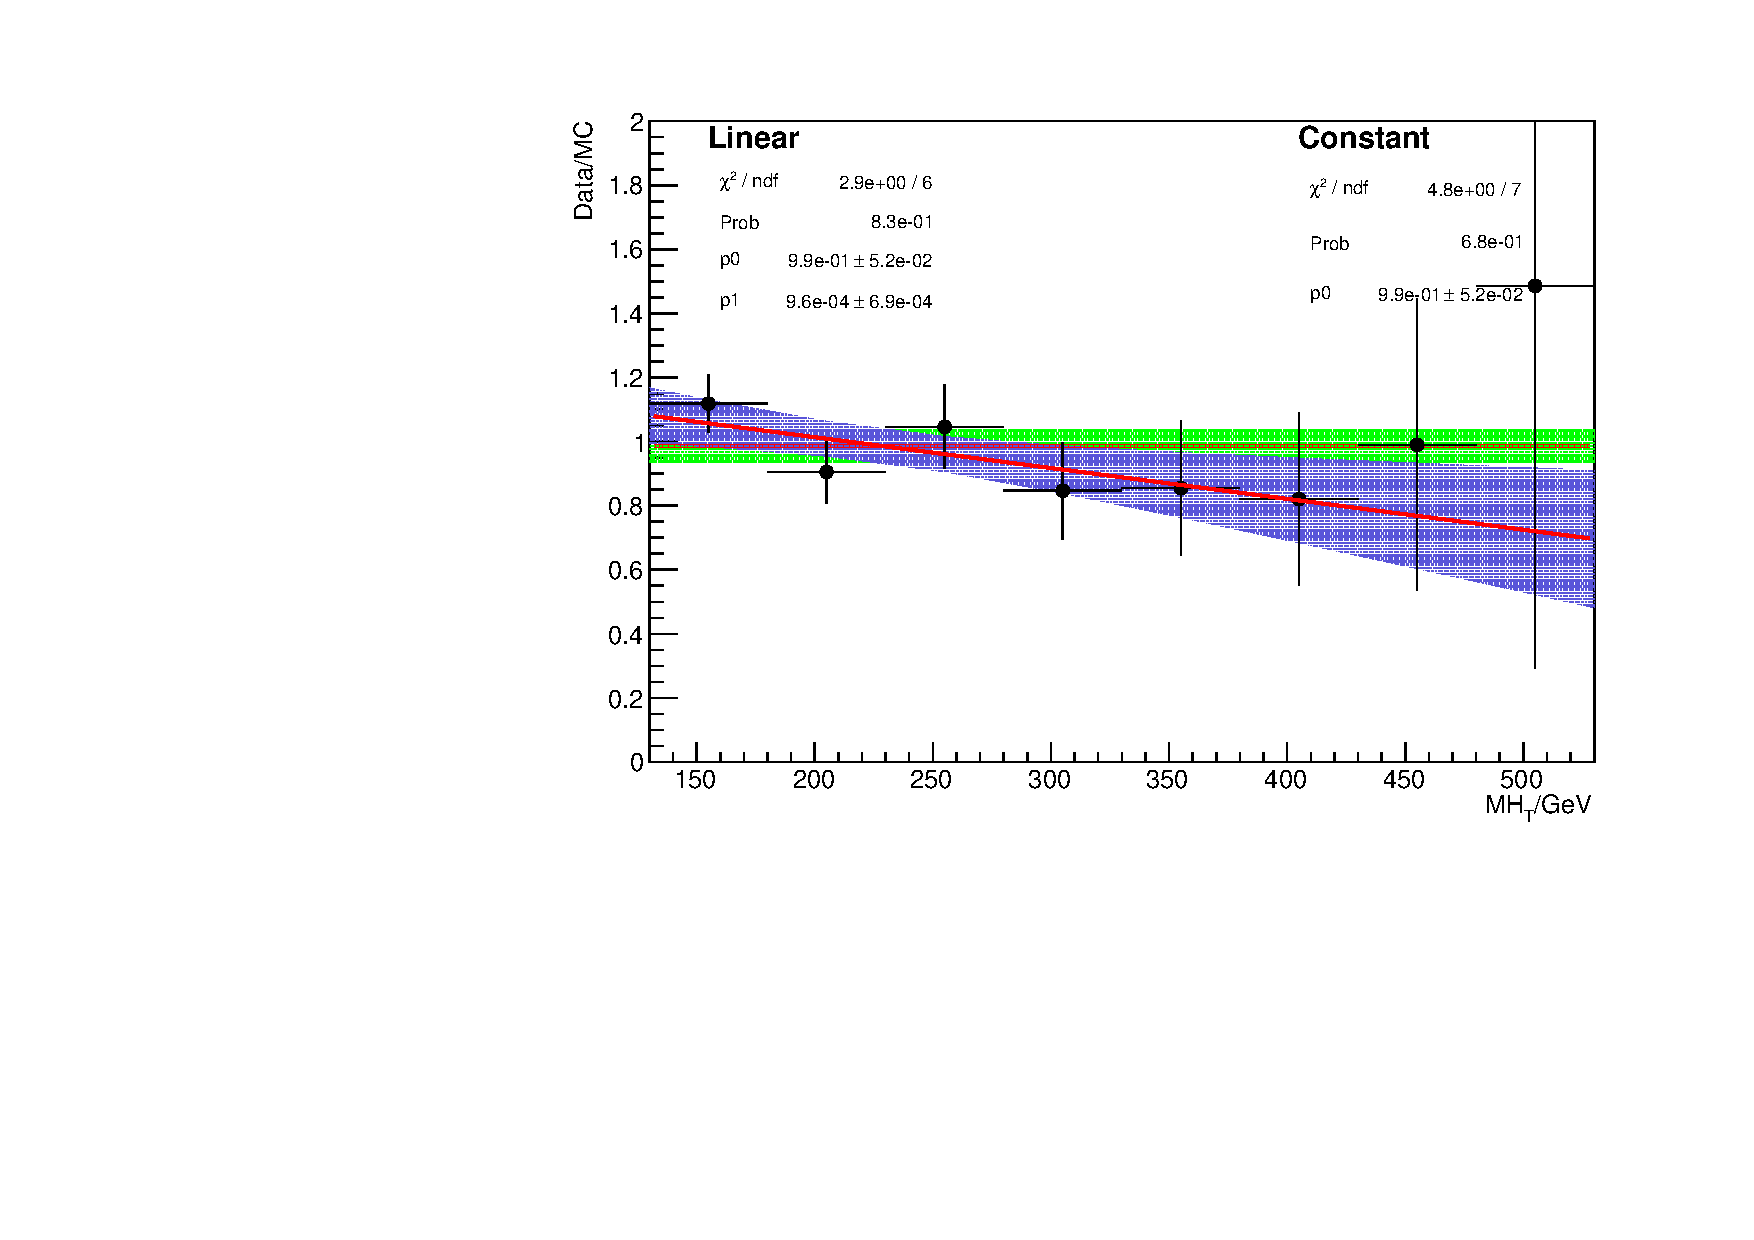
\includegraphics[width=0.5\textwidth]{figures/template/linear/mht_eq0b_ge4j_ht_475_575_SingleMu.pdf}
  }~~
  \\
  \caption{\label{fig:linearFits0bGe4} 
  The data/MC distribution against \mht for the 0b, $\ge4$j category and \ht 475-575\GeV bin.
  The large linear bias in the linear component seen in \ref{fig:linearMotiv} is
  largely mitigated.
}
\end{figure}

\begin{figure}[h!]
  \centering
  \subfigure[\gj]{
    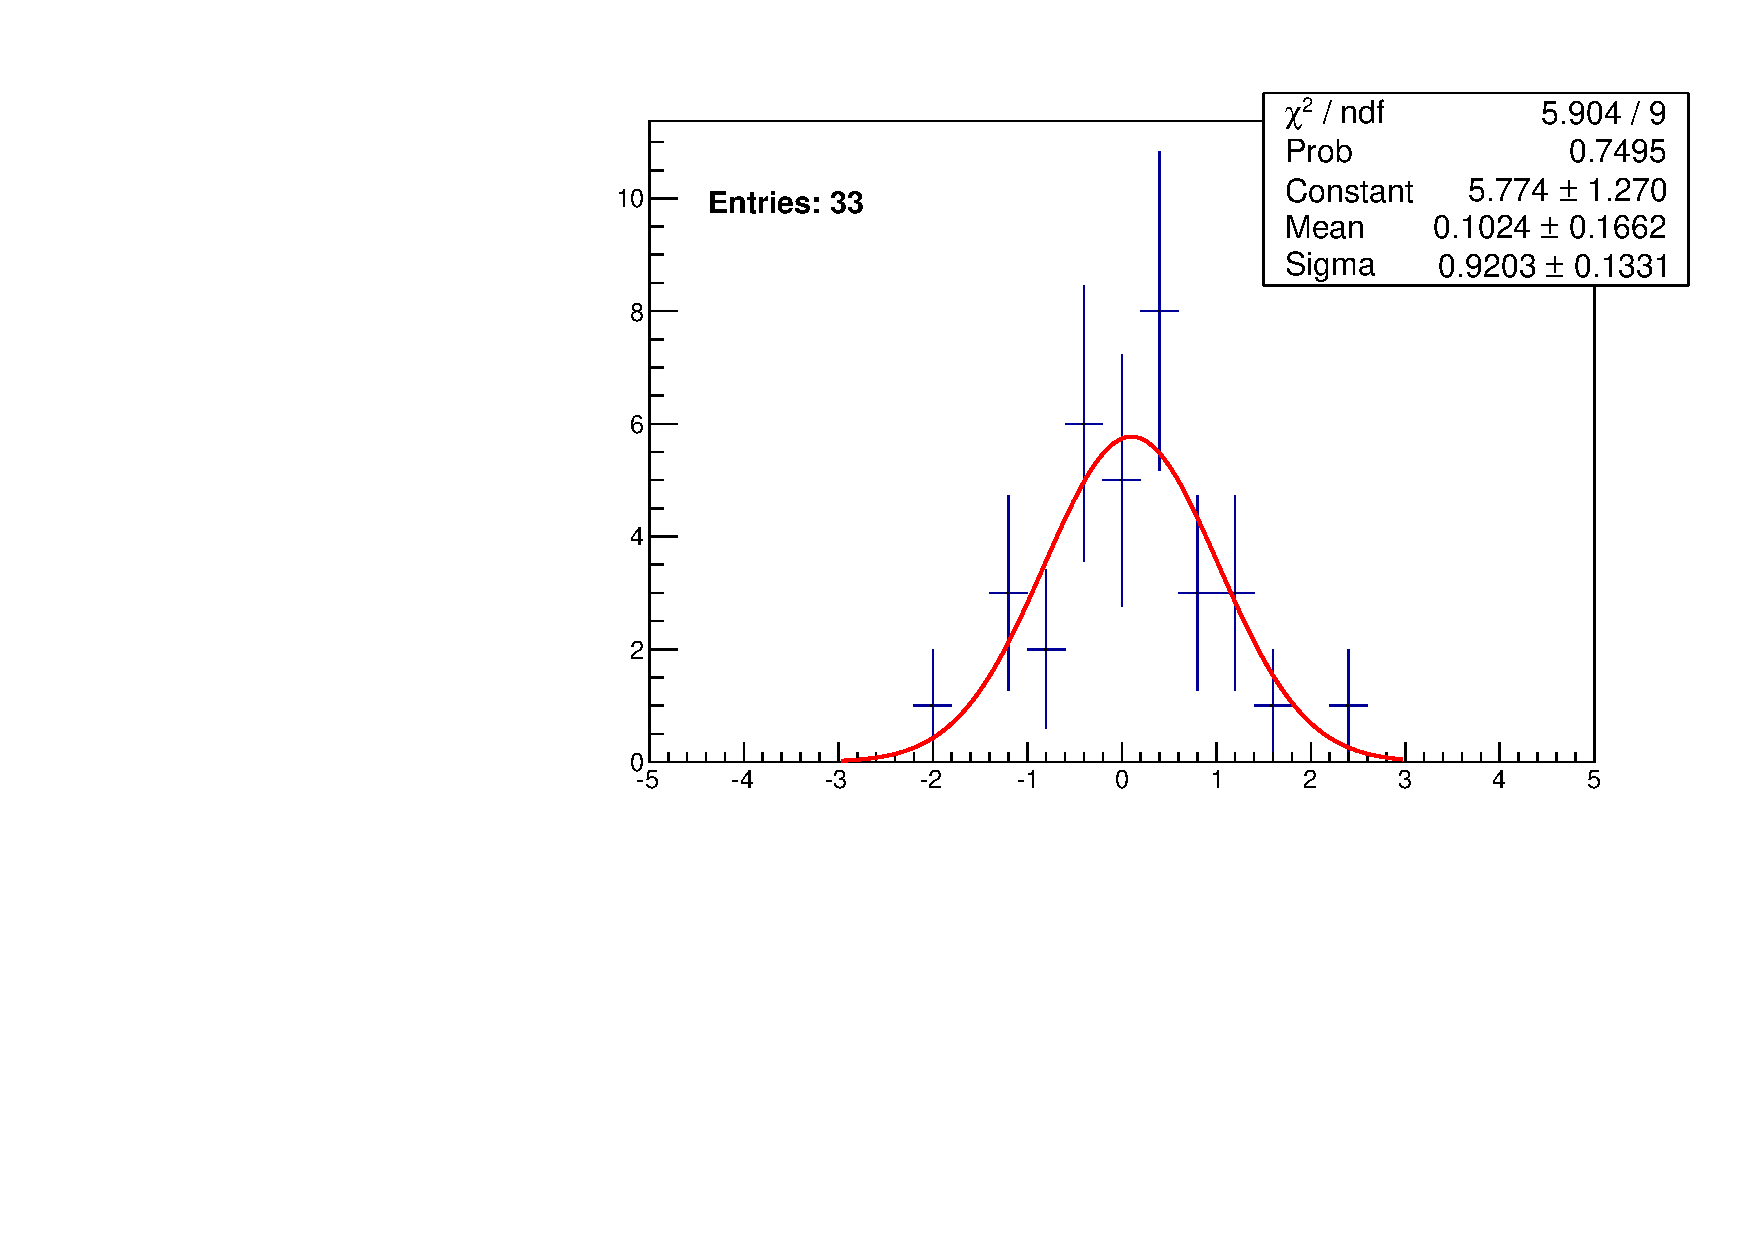
\includegraphics[width=0.5\textwidth]{figures/template/linear/pull_Linear2D_p1_SinglePhoton.pdf}
  }~~
  \subfigure[\mmj]{
    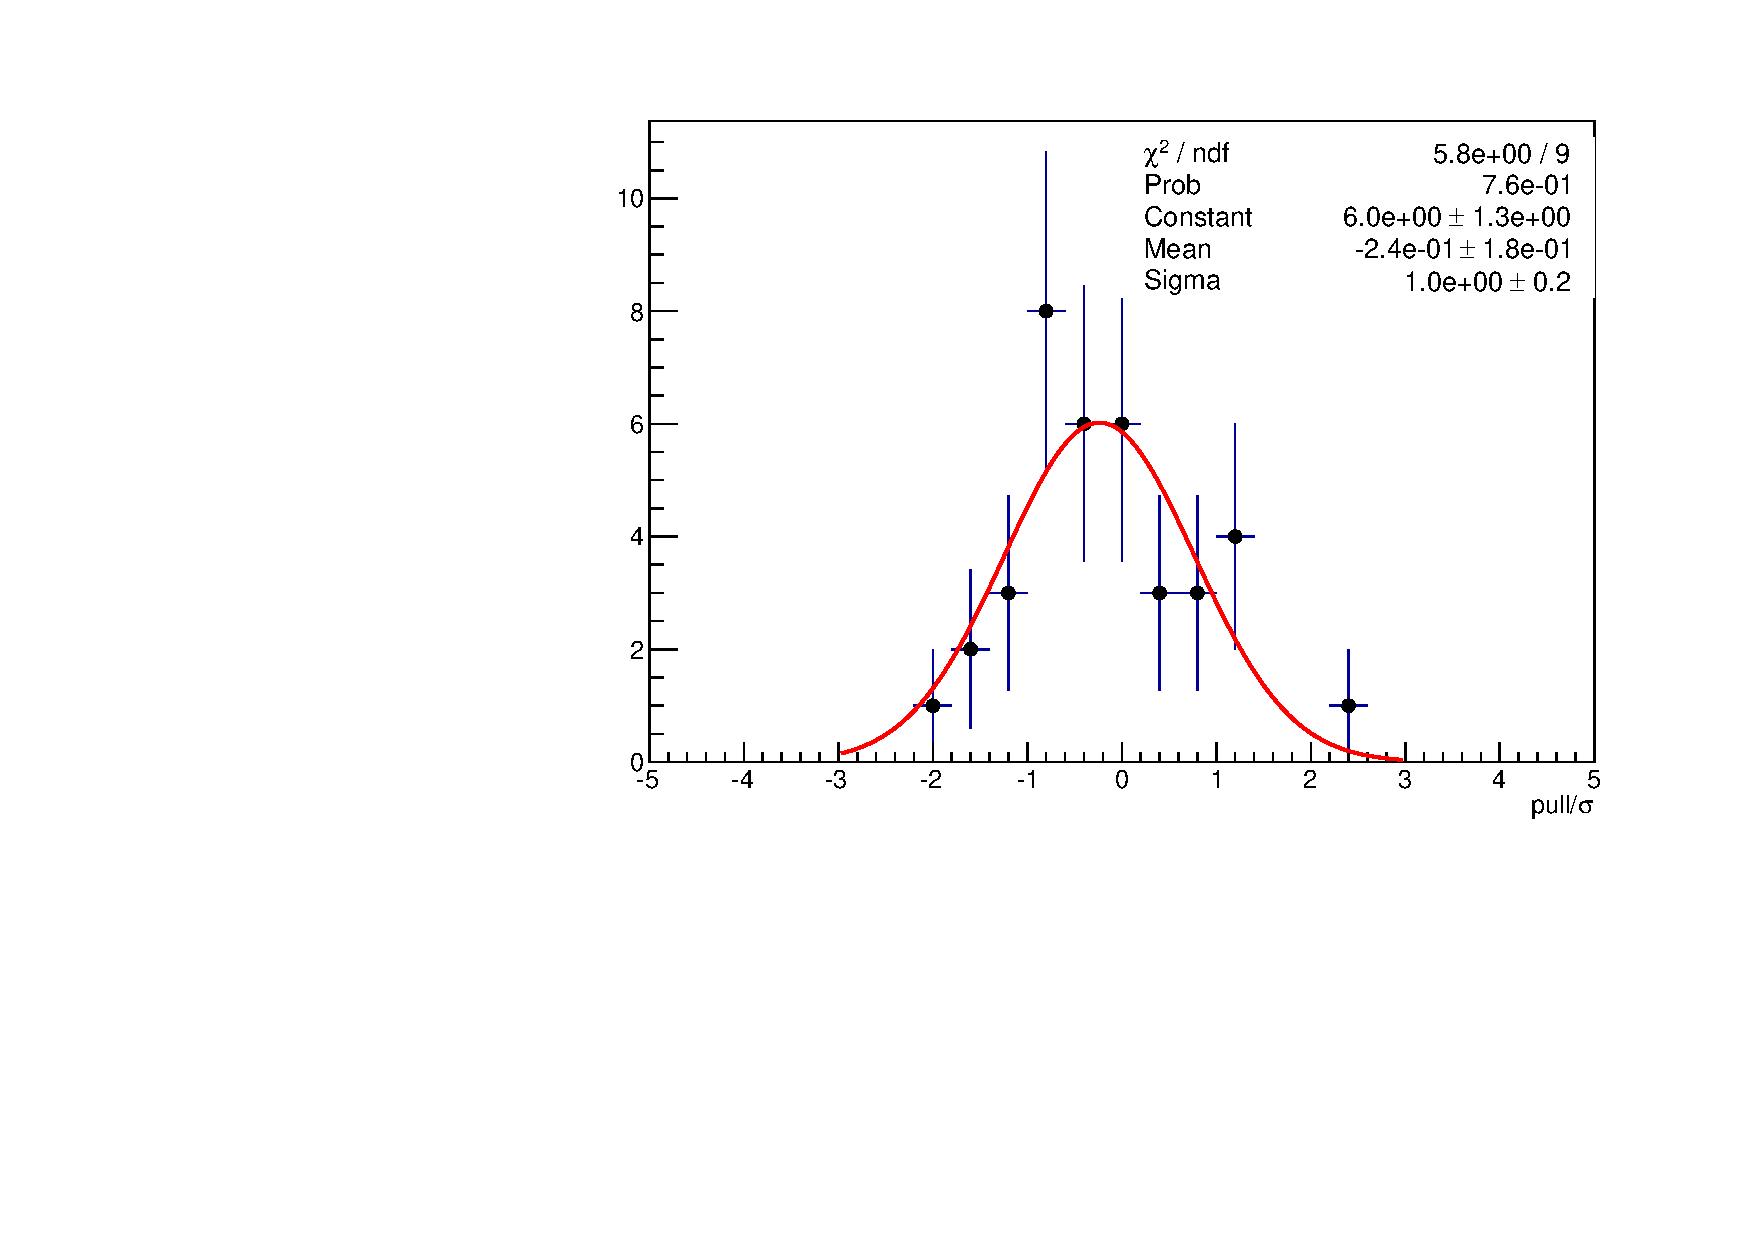
\includegraphics[width=0.5\textwidth]{figures/template/linear/pull_Linear2D_p1_DoubleMu.pdf}
  }\\
  \subfigure[\mj]{
    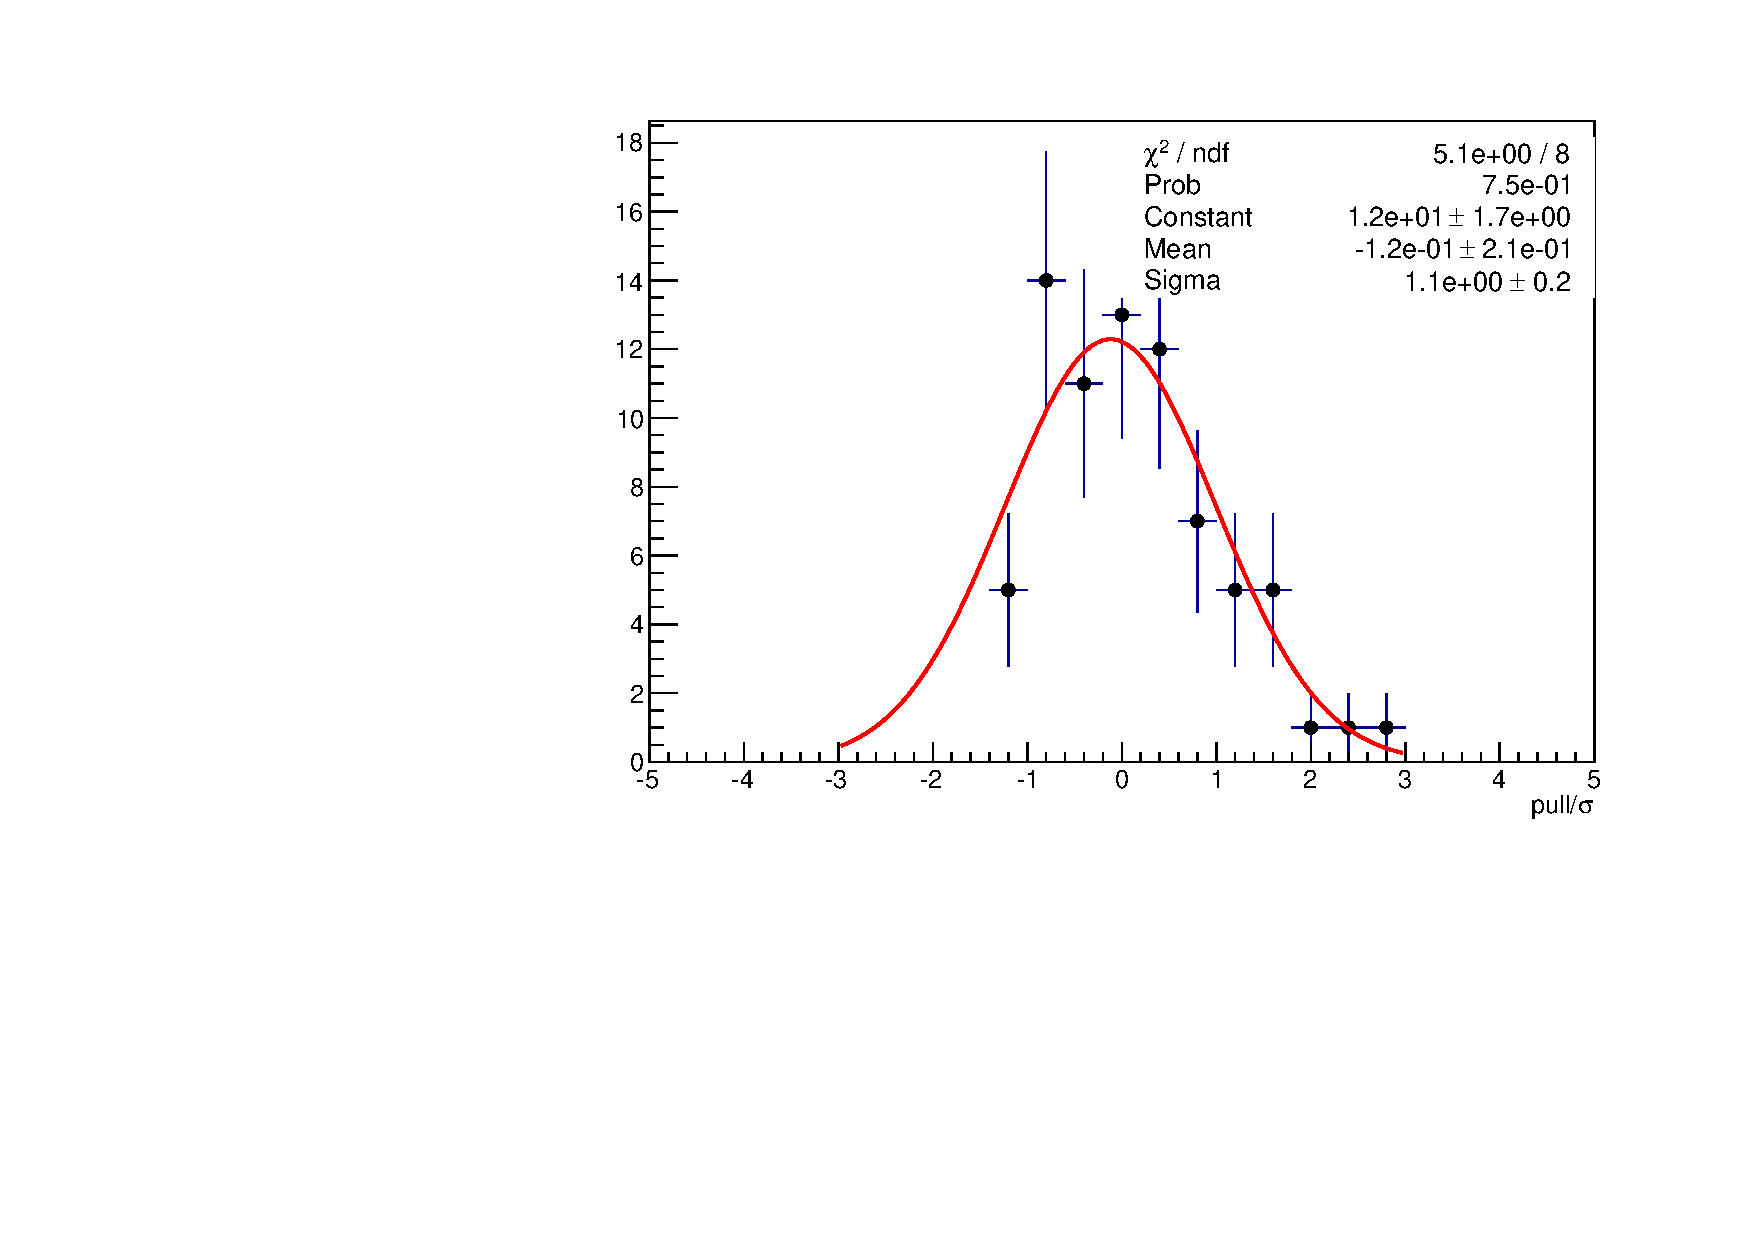
\includegraphics[width=0.5\textwidth]{figures/template/linear/pull_Linear2D_p1_SingleMu.pdf}
  }~~
  \\
  \caption{\label{fig:pulls} 
  The pull distribution of the linear parameter from the flat hypothesis showing
  a distribution consistent with mean and sigma of zero and one. 
  This is consistent with the zero bias hypothesis.
}
\end{figure}
\begin{figure}[h!]
  \centering
  \subfigure[\gj]{
    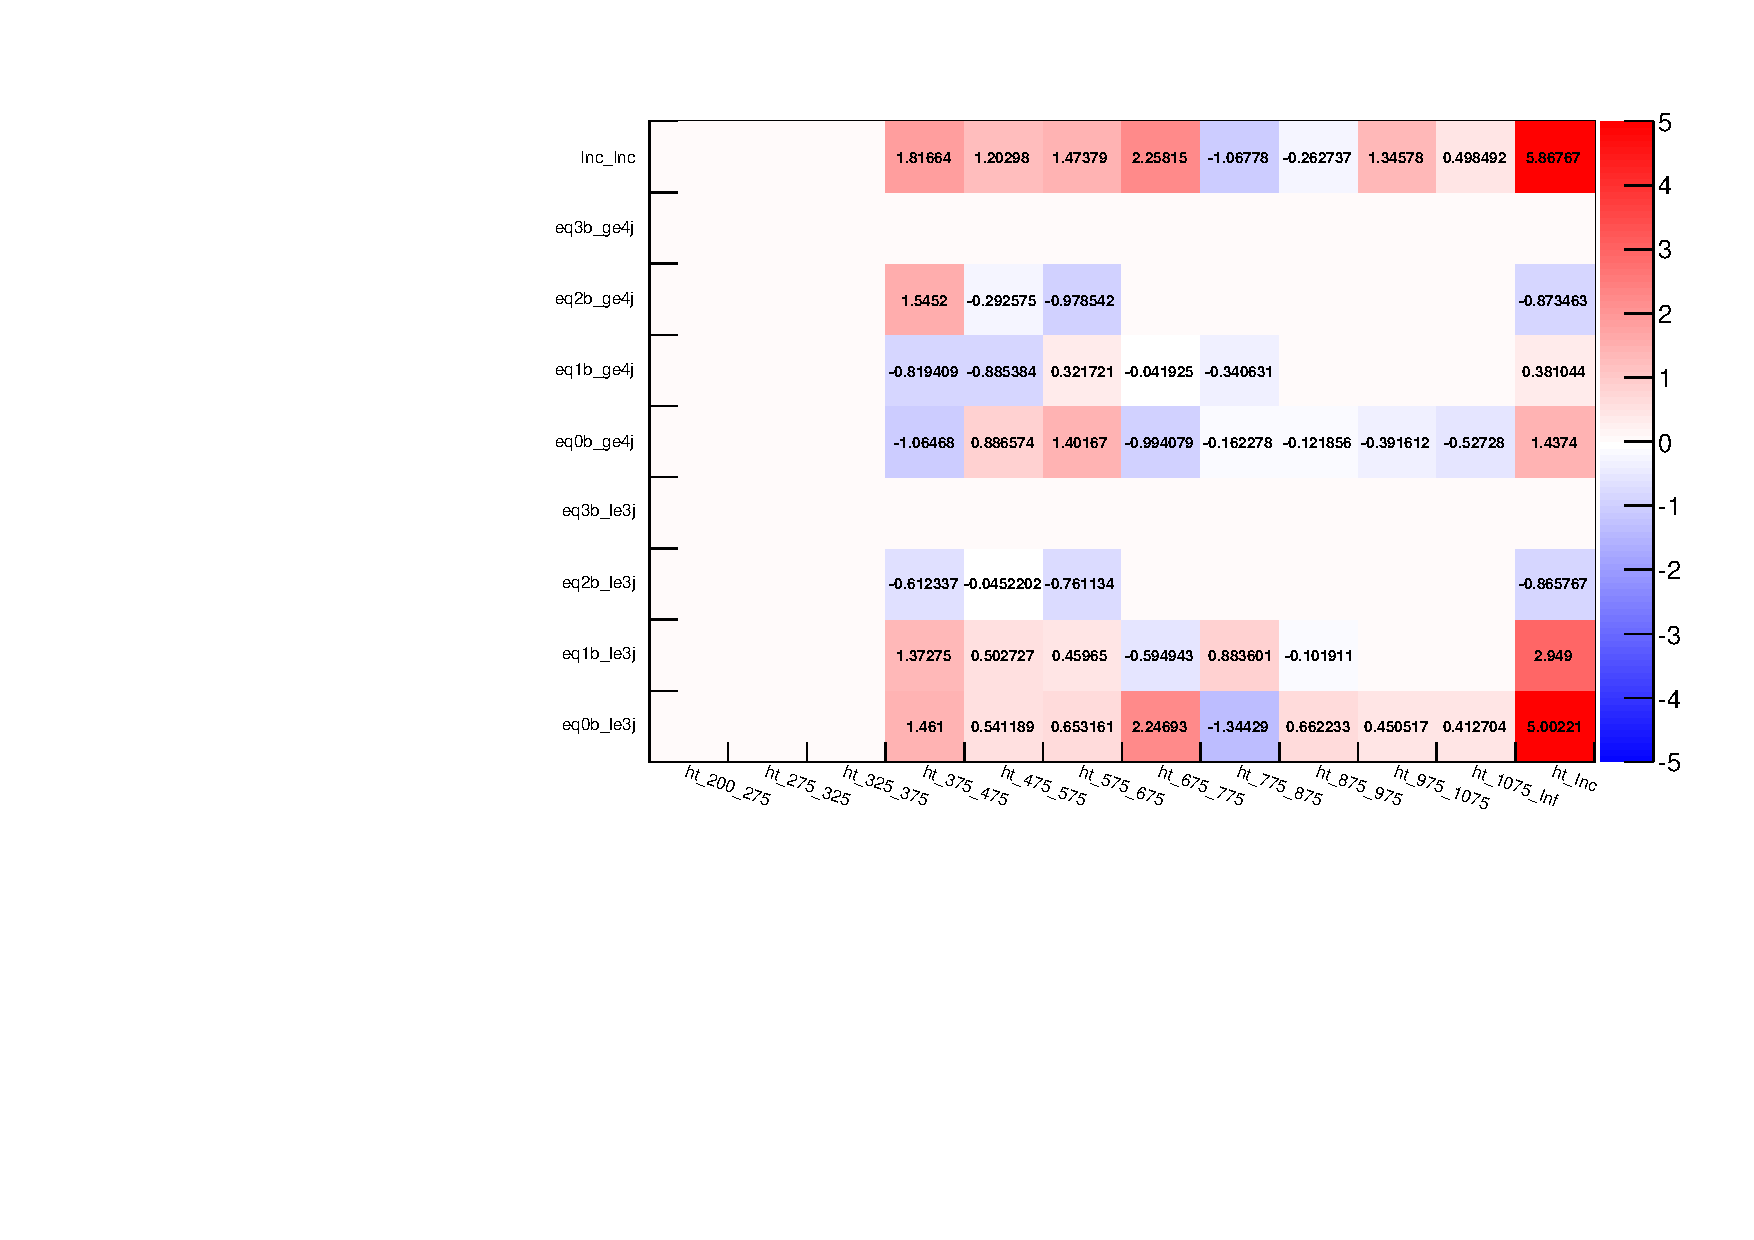
\includegraphics[width=0.5\textwidth]{figures/template/linear/frenchFlagPull_Linear2D_p1_SinglePhoton.pdf}
  }~~
  \subfigure[\mmj]{
    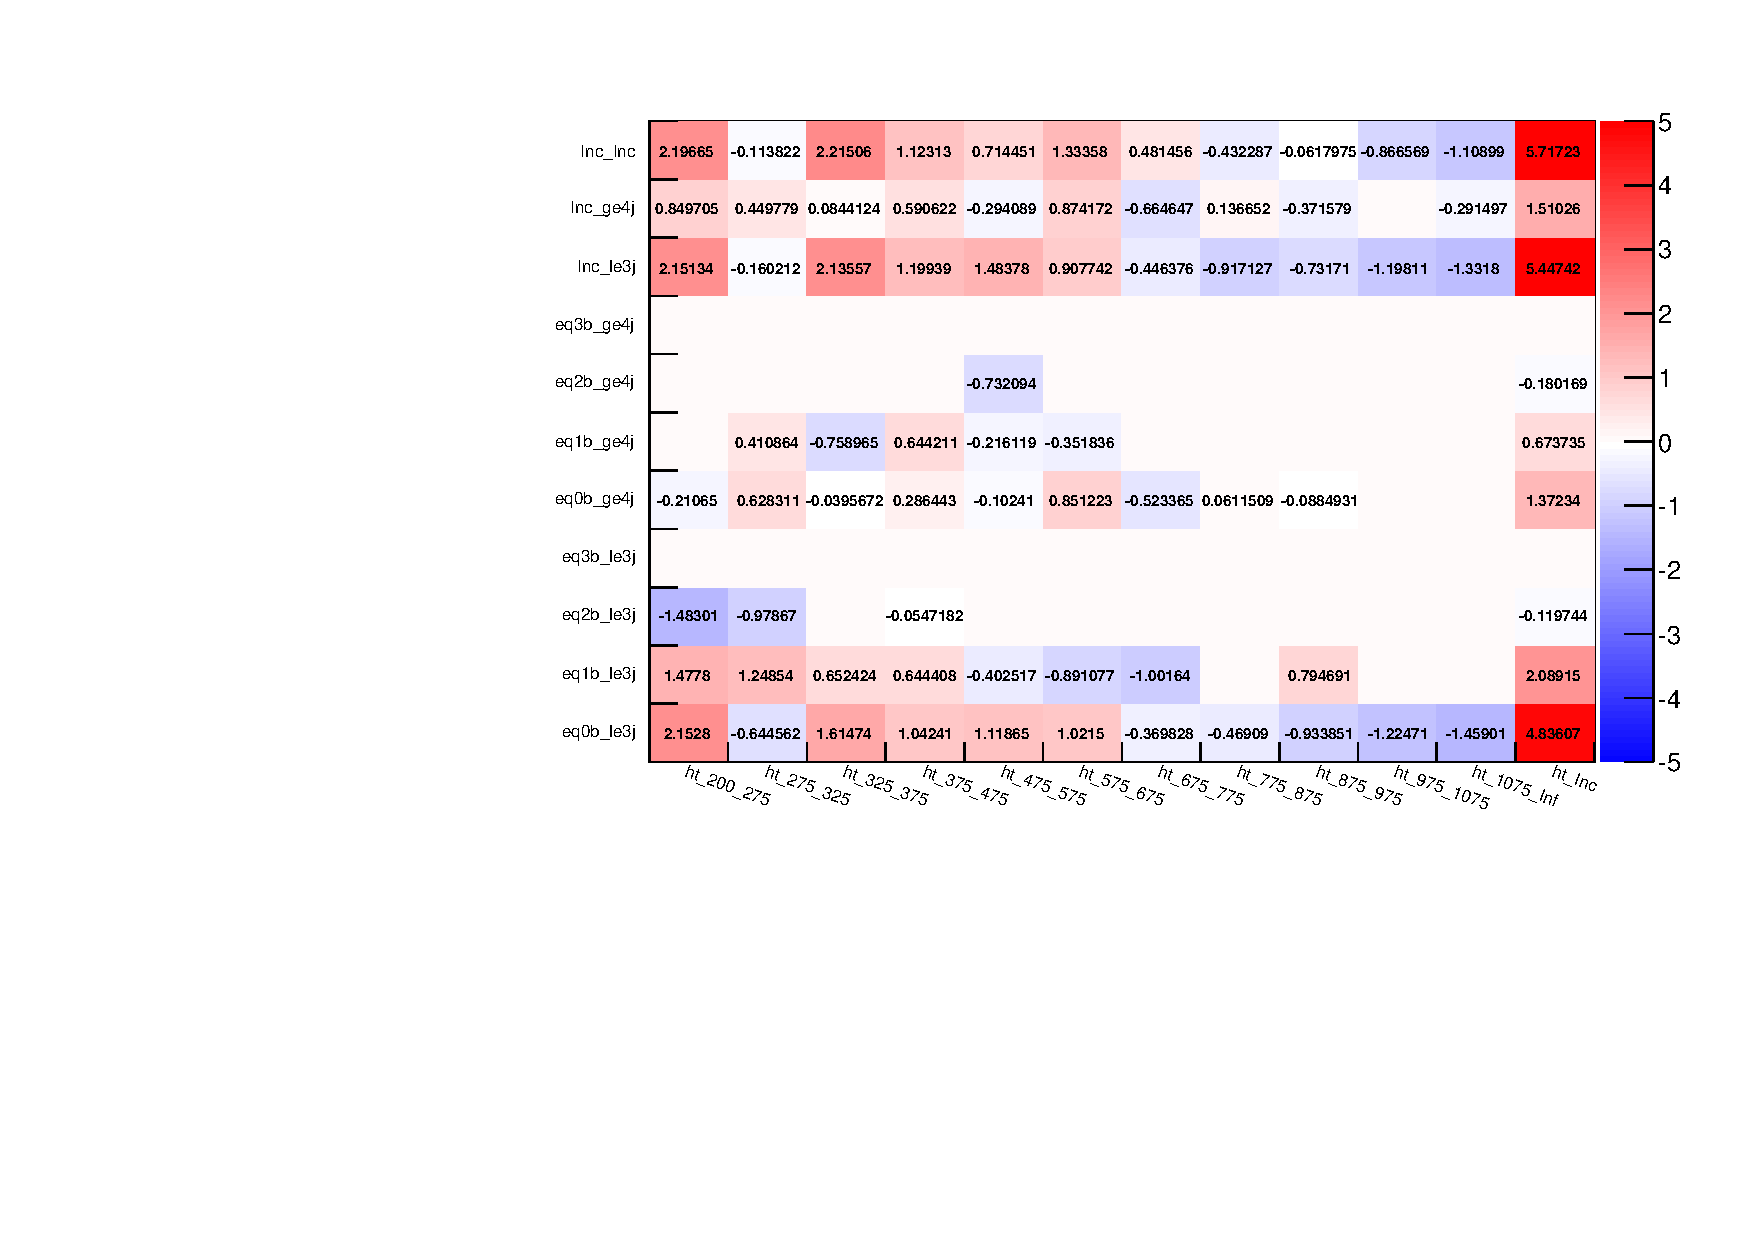
\includegraphics[width=0.5\textwidth]{figures/template/linear/frenchFlagPull_Linear2D_p1_DoubleMu.pdf}
  }\\
  \subfigure[\mj]{
    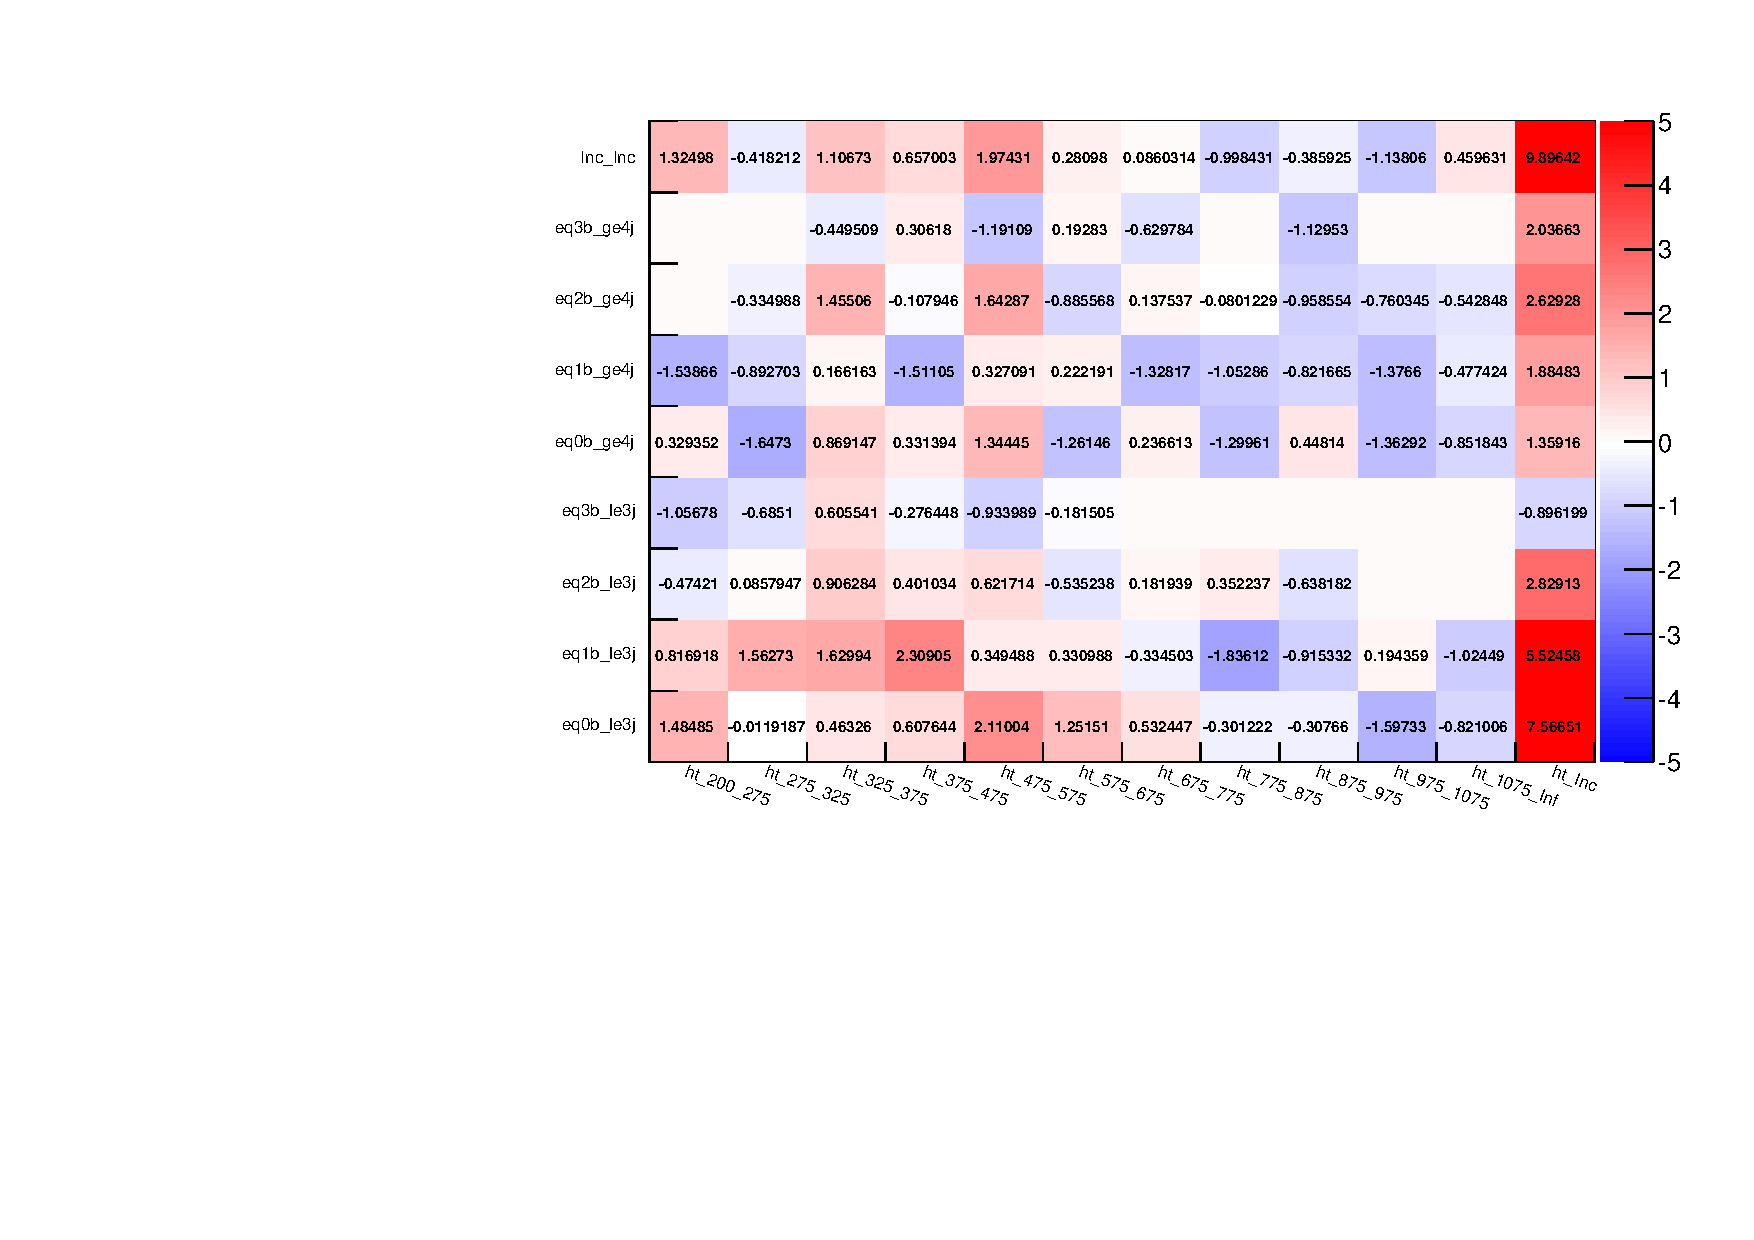
\includegraphics[width=0.5\textwidth]{figures/template/linear/frenchFlagPull_Linear2D_p1_SingleMu.pdf}
  }~~
  \\
  \caption{\label{fig:frenchFlagPulls} 
  The pull distribution of the linear parameter from the flat hypothesis across all
  \ht bins and categories. There are no significant pulls for the \ht binned
  fits while the \ht inclusive case shows very large pulls as expected. 
  Due to trigger requirements the \gj control sample may only be used for \ht > 375\GeV.

}
\end{figure}

%Stuff from old chapter
% \subsection{Systematic uncertainties in the \mht dimension\label{sec:syst-on-shape}}
%
%
% Several potential sources of uncertainty will be considered, such as
% ISR, JES, PDF, b-tag scale factors, etc, as detailed below. In
% general, for each source of systematic, the \mht templates are found
% based on $\pm$1$\sigma$ variations in the relevant source of
% uncertainty. The alternative templates reflect the magnitude of the
% migration of events between bins in \mht (but not in \njet, \nb, nor
% \scalht, which is encapsulated by the normalisation systematic
% uncertainties from closure tests). If the systematic source is found
% to be significant, the template variations will be included in the
% likelihood. 
%
% \begin{figure}[]
%   \centering
%   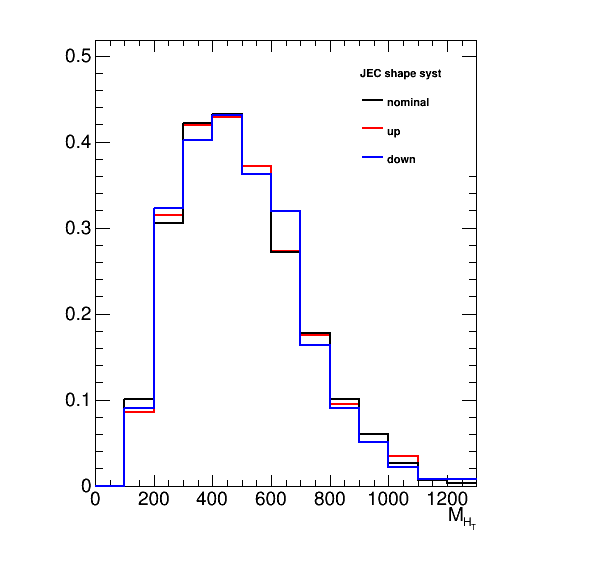
\includegraphics[width=0.5\textwidth]{figures/closureTests/mhtJetSyst_SMS_T1bbbb_2J_mGl1000_mLSP900_JEC_ge3b_ge5j_800_1600.png}
%   \caption{\label{fig:jec-shape} Alternative \mht templates that
%     refect uncertainties in the jet energy scale corrections for
%     $\geq$5 jets, $\geq$3 b-jets, and $\scalht > 800\gev$ bin for the
%     10 \ifb luminosity scenario.}
% \end{figure}
%
% An indicative behaviour is shown in Figure~\ref{fig:jec-shape} by
% considering the variation of jet energy scale given the uncertainties
% determined in Run~1. The relative change in the \mht distribution is
% determined when varying the energy of all jets in an event up or down
% according to a \pt- and $\eta$-dependent jet energy scale uncertainty
% (\ie vary the event scale up and down), as recommended by the JetMET
% POG. 
%
% \begin{figure}[]
%   \centering
%   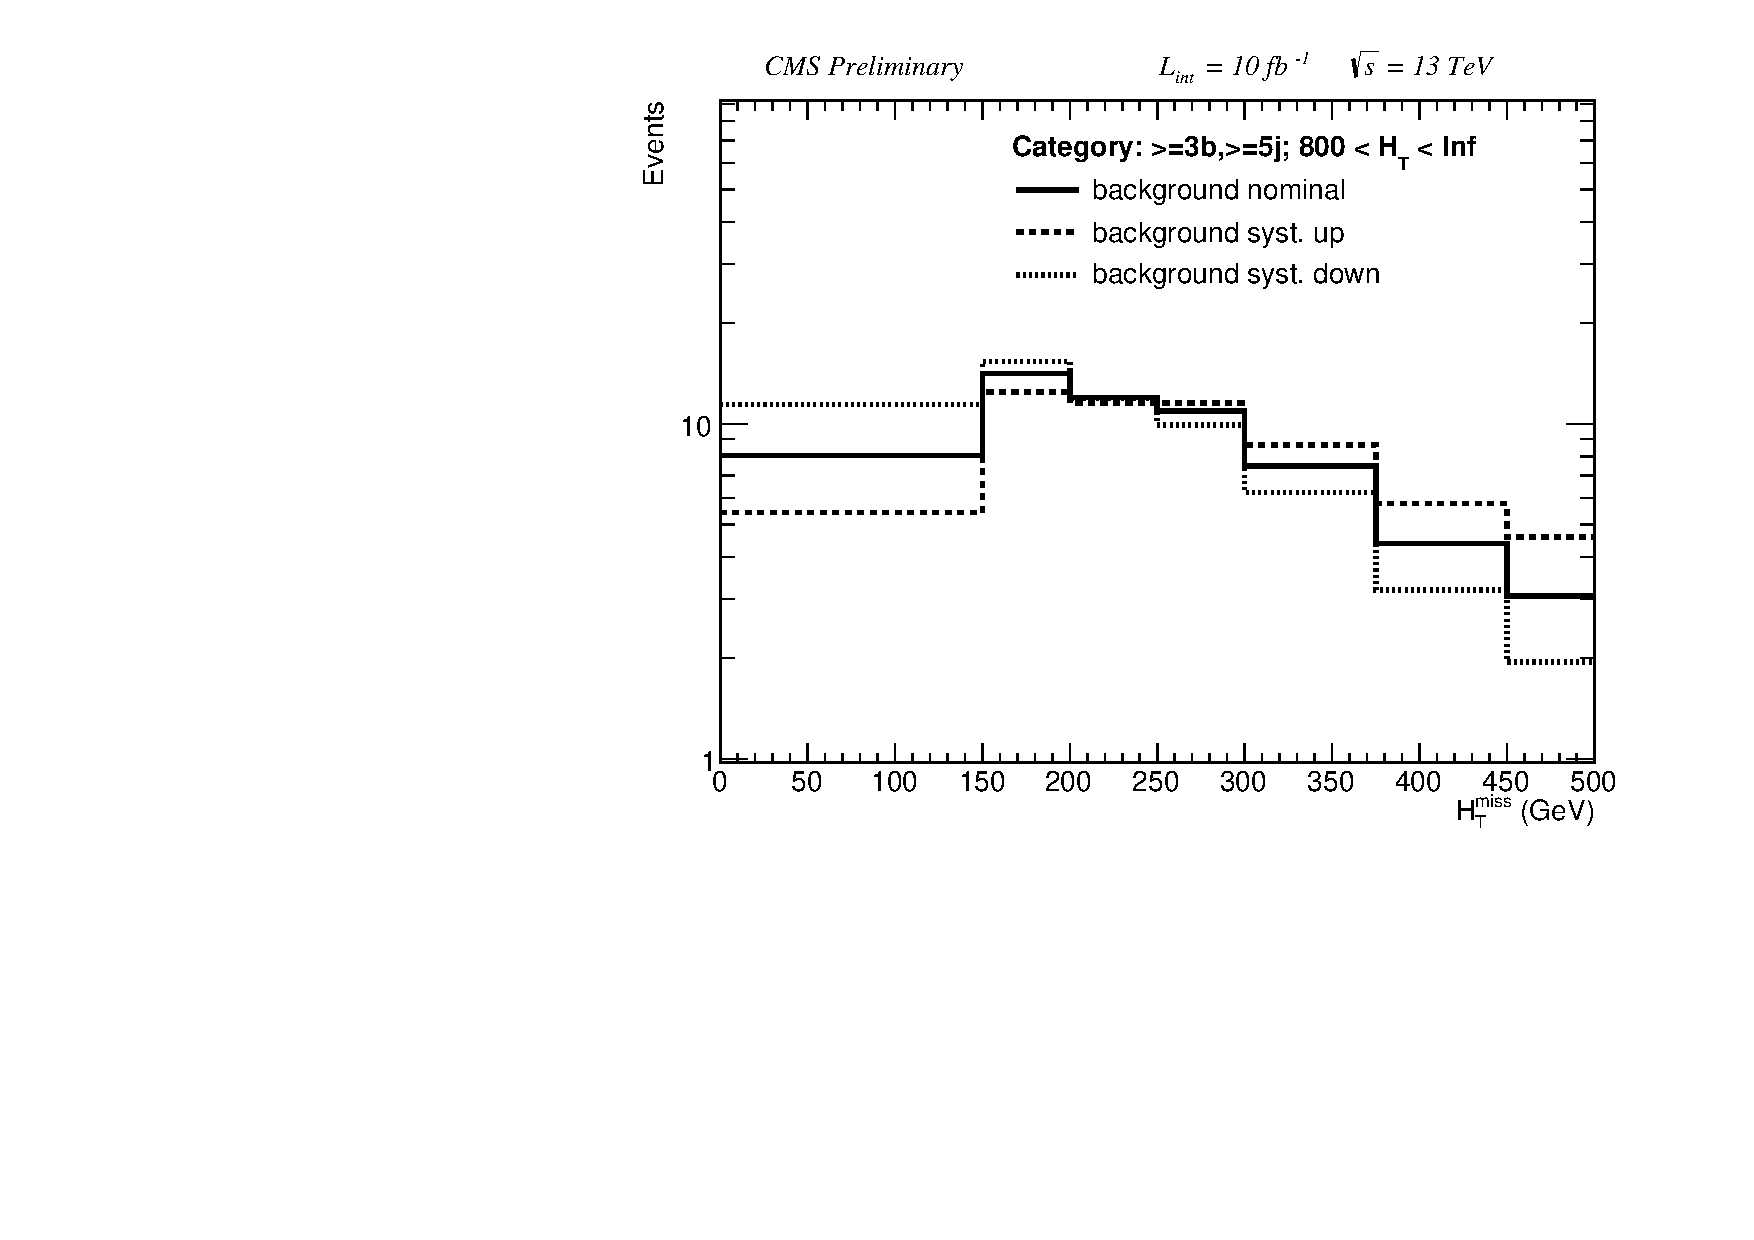
\includegraphics[width=0.7\textwidth]{figures/mhtShapeSyst/MHTShapeSyst_ge3b_ge5j_800_Inf.pdf}
%   \caption{\label{fig:mht-shape-syst-toy} 
%     The nominal \mht shape and its up/down alternative shapes for the \ttbar/W background in the $\njet \geq5$, $\nb \geq 3$
%     category for the $\HT > 800 \gev$ bin.
%   }
% \end{figure}
%
% For the sensitivity studies reported in the AN, we assume a significant 
% uncertainty on the distribution of events in the \mht dimension. 
% At present this is modelled assuming a maximum of 50\% uncertainty in the last \mht bin, 
% which typically represents the bin with the best single sensitivity in a given \scalht category. 
% In this model the systematic uncertainty of lower \mht bins is determined 
% as an exponential with a maximum shift of 50\% in the last \mht bin. 
% Figure \ref{fig:mht-shape-syst-toy} shows the corresponding $\pm$1 Sigma variation of the 
% \mht template obtained from this systematic model. 
% As can be seen, this variation is much larger than the ones induced by MC variations (Figure \ref{fig:jec-shape}).  
% We also have tested other models of the \mht systematic such as a linear instead of an exponential function which lead to rather similar results. 
%
% Finally, studies are underway with the aim of establishing procedures
% based on data (akin to the closure tests) that will help to either
% estimate dominant source of uncertainty related to how events are
% distributed in \mht, or to at least provide data-driven cross checks.
% An attempt to avoid a reliance solely on variations in simulation is
% considered important for a discover-orientated analysis. The current
% ongoing studies are based on Run~1 data.
%
% %While simulation-based studies are also ongoing, some comments are
% %made below on some of the potential sources of uncertainty that are
% %expected to be dominant. This list is clearly not exhaustive.
% %
% %{\bf Jet energy scale:} 
% %
%
% %
% %{\bf PDF uncertainties:}
% %
% %\newcommand{\lcr}{Left: $\frac{\epsilon_{CTEQ6L1}}{\epsilon_{CT10}}$,
% %  center: $\frac{\epsilon_{CTEQ6L1}}{\epsilon_{MSTW08}}$, right:
% %  $\frac{\epsilon_{CTEQ6L1}}{\epsilon_{NNPDF2.1}}$}
% %
% %The samples are produced with the \verb!CTEQ6L1! PDF set by default.
% %The shape is compared with that obtained with three alternative PDF
% %sets: \verb!CT10!, \verb!NNPDF2.1!, and \verb!MSTW2008!. The envelope
% %and its uncertainties are determined following the PDF4LHC
% %recommendation~\cite{pdf4lhc}. 
% %
% %{\bf Initial state radiation:}
% %
% %Will have to cook up a recipe for this\ldots
% %
% %
% %{\bf \texorpdfstring{\mht/\met}{MHT/MET} cleaning cut:}
% %
% %The efficiencies for the requirement $\mht/\met < 1.25$ must be
% %measured in data and simulation as a function of \mht for each \scalht
% %bin. The ratio of these two efficiencies should be unity. Deviation
% %from unity is taken to represent the uncertainties on the simulation
% %modelling of this variable for processes with significant, genuine
% %\met. This can be used to define templates for the uncertainty on this
% %quantity.
% %
% %{\bf Dead ECAL filter:}
% %
% %The ratio of efficiencies observed in data and simulation for the dead
% %ECAL filter may be used as in Section~\ref{sec:sms-syst-mht-met} to
% %templates for the uncertainty from the Dead ECAL filter.
